\chapter{Numerical Methods}

\section{Monte Carlo}

A discussion of the Monte Carlo methods here



\section{Incoherent Scatter Spectra Calculation}

\subsection{Obtaining $M_s$ and $\chi_s$}

The incoherent scatter spectra of a plasma is calculated using Eq.~\ref{eq:scattering-spectra}, which needs Eqs.~\ref{eq:dielectric}-\ref{eq:Ms}.
For an arbitrary distribution function, it is difficult to calculate this, especially when the distribution function does not have an analytical form (like that of a Monte Carlo output).
\cite{goodwin2018} provide a method involving applying several curve fitting techniques to the ion distribution function. 
This method provides good results but requires significant input from the user to ensure a good fit. % Double check this statement. 
The primary reason for these techniques was to have minimal noise in the derivative of the distribution, as used in Eq.~\ref{eq:chis} and described in Eq.~\ref{eq:chis_derivative}.
Furthermore, the spectrum calculation in \citep{goodwin2018} assumes tha the ions are entirely unmagnetized. 
We will provide a different method with no input from the user (beyond choosing the initial velocity mesh extent and resolution) that fully include the effects of collisions and magnetic fields.


To simplify the calculation, we assume that the distribution function is axisymmetric in velocity space about the axis parallel to the magnetic field. 
Thus, cylindrical coordinates are the natural choice with the velocity space discretized by $v_\parallel$ and $v_\perp$ and the azimuth angle described by $\phi$.
The integral over all velocity space of an arbitrary function $f$ in cylindrical coordiantes is
\begin{equation}
	\int f(\mathbf{v}) d\mathbf{v} = \int_0^\infty  dv_\perp v_\perp  \int_{-\infty}^\infty dv_\parallel \int_0^{2\pi} f(v_\perp, v_\parallel) d\phi.
	\label{eq:cylindrical_integration}
\end{equation}
Due to azimuthal symmetry, the integral over $\phi$ just becomes $2\pi$ yielding
\begin{equation}
	\int f(\mathbf{v}) d\mathbf{v} = 2\pi \int_0^\infty  dv_\perp v_\perp  \int_{-\infty}^\infty f(v_\perp, v_\parallel)  dv_\parallel.
	\label{eq:cylind_int_2pi}
\end{equation}


Eq.~\ref{eq:cylind_int_2pi} can be applied to the calculation of $U_s$, $M_s$, and $\chi_s$. 
Let us begin with $U_s$. We can rewrite the denominator to be $v_\parallel-z$ where 
\begin{equation}
	z = \frac{\omega - n\Omega_{cs}- i \nu_s}{k_\parallel}.
	\label{eq:z}
\end{equation}
Using Eqs.~\ref{eq:cylind_int_2pi} and \ref{eq:z}, Eq.~\ref{eq:Us} becomes
\begin{equation}
	U_s = - \frac{2 \pi i \nu_s}{k_\parallel} \sum_n 
	\int_0^\infty dv_\perp v_\perp J_n^2 \bigg( \frac{k_\perp v_\perp}{\Omega_{cs}} \bigg)
	\int_{-\infty}^\infty  
	\frac{f_{0s}(v_\perp, v_\parallel)}{v_\parallel - z} dv_\parallel
	\label{eq:Us_final}
\end{equation}


For $M_s$, the denominator term can similarly be rewritten as $(v_\parallel-z)(v_\parallel-z^*)$
where $z^*$ is the complex conjugate of $z$.
Therefore, Eq.~\ref{eq:Ms} can be rewritten as  % Revisit this calculation and make sure I'm doing it correctly. I feel like to do it right, I need a kpar^2 in the outside denominator
\begin{equation}
	M_s = \frac{\nu_s}{|1+U_s|^2} 
	\Bigg[ -\frac{|U_s|^2}{\nu_s^2} 
	+ \frac{1}{k_\parallel^2}\sum_n \int_0^\infty   dv_\perp v_\perp J_n^2 \bigg( \frac{k_\perp v_\perp}{\Omega_{cs}} \bigg)
	\int_{-\infty}^\infty \frac{f_{0s}(v_\perp, v_\parallel)}{(v_\parallel - z)(v_\parallel - z^*)} dv_\parallel
	\Bigg]
	\label{eq:Ms_final}
\end{equation}


The denominator term for the magnetized susceptibility, $\chi_s$, can also be rewritten as $v_\parallel-z$, just as we did for $U_s$ in Eq.~\ref{eq:Us_final}.
Therefore, Eq.~\ref{eq:chis} can be rewritten as
\begin{equation}
	\chi_s = -\frac{\omega_{ps}^2}{k_\parallel k^2 (1+U_s)} \sum_n \int d\mathbf{v}^3 
	 \frac{ J_n^2\Big( \frac{k_\perp v_\perp}{\Omega_{cs}}\Big)  }{v_\parallel-z}
	\bigg( k_\parallel \frac{\partial}{\partial v_\parallel} + \frac{n\Omega_{cs}}{v_\perp} \frac{\partial }{\partial v_\perp}  \bigg) f_{0s}(v_\perp, v_\parallel) .
	\label{eq:chis_denom}
\end{equation}
Let us split this integral into two integrals based on the derivatives:
\begin{align}
	\chi_s^\parallel &= -\frac{\omega_{ps}^2}{k^2 (1+U_s)} \sum_n \int d\mathbf{v}^3 
	\frac{ J_n^2\Big( \frac{k_\perp v_\perp}{\Omega_{cs}}\Big)  }{v_\parallel-z}
	\frac{\partial}{\partial v_\parallel} f_{0s}(v_\perp, v_\parallel)
	\label{eq:chis_par} \\
	\chi_s^\perp &= -\frac{\omega_{ps}^2}{k_\parallel k^2 (1+U_s)} \sum_n \int d\mathbf{v}^3 
	\frac{ J_n^2\Big( \frac{k_\perp v_\perp}{\Omega_{cs}}\Big)  }{v_\parallel-z}
	\frac{n\Omega_{cs}}{v_\perp} \frac{\partial }{\partial v_\perp} f_{0s}(v_\perp, v_\parallel).
	\label{eq:chis_perp}
\end{align}
These derivatives are difficult to deal with numerically.
So, we want to use integration by parts to move the derivative from the distribution function to other things that we already know the analytical derivatives of.

First, we look at the parallel susceptibility.
In cylindrical coordinates, it becomes
\begin{equation}
	\chi_s^\parallel = -\frac{2\pi \omega_{ps}^2}{k^2 (1+U_s)} \sum_n 
	\int_0^\infty dv_\perp v_\perp J_n^2 \bigg( \frac{k_\perp v_\perp}{\Omega_{cs}}  \bigg)
	\int_{-\infty}^\infty \frac{1}{v_\parallel-z} 
	\frac{\partial}{\partial v_\parallel} f_{0s}(v_\perp, v_\parallel).
	\label{eq:chis_par_cylind}
\end{equation} 	
Using integration by parts, the parallel integral becomes
\begin{equation}
	\int_{-\infty}^\infty \frac{1}{v_\parallel-z} 
	\frac{\partial}{\partial v_\parallel} f_{0s}(v_\perp, v_\parallel) = 
	\frac{f_{0s}(v_\parallel,v_\perp)}{v_\parallel-z}\bigg|_{-\infty}^\infty
	- \int_{-\infty}^\infty dv_\parallel f_{0s}(v_\perp, v_\parallel)
	\frac{\partial}{\partial v_\parallel} \bigg( \frac{1}{v_\parallel-z}  \bigg).
	\label{eq:par_int_parts}
\end{equation}
The boundary term is zero because the distribution function tends to 0 at $\pm \infty$.
The remaining derivative is straightforward to calculate resulting in a parallel integral of 
\begin{equation}
	\int_{-\infty}^\infty \frac{1}{v_\parallel-z} 
	\frac{\partial}{\partial v_\parallel} f_{0s}(v_\perp, v_\parallel) = 
	\int_{-\infty}^\infty \frac{f_{0s}(v_\perp, v_\parallel)}{(v_\parallel-z)^2}  dv_\parallel.
	\label{eq:par_int_parts_final}
\end{equation}
Substituting Eq.~\ref{eq:par_int_parts_final} into Eq.~\ref{eq:chis_par_cylind} gives a parallel susceptibility of
\begin{equation}
	\chi_s^\parallel = -\frac{2\pi \omega_{ps}^2}{k^2 (1+U_s)} \sum_n 
	\int_0^\infty dv_\perp v_\perp J_n^2 \bigg( \frac{k_\perp v_\perp}{\Omega_{cs}}  \bigg)
	\int_{-\infty}^\infty \frac{f_{0s}(v_\perp, v_\parallel)}{(v_\parallel-z)^2} dv_\parallel.
	\label{eq:chis_par_final}
\end{equation}

Now, let us look at the perpendicular integral. In cylindrical coordinates, Eq.~\ref{eq:chis_perp} is
\begin{equation}
	\chi_s^\perp = -\frac{2\pi \omega_{ps}^2}{k_\parallel k^2 (1+U_s)} \sum_n
	n \Omega_{cs} 
	\int_{-\infty}^\infty \frac{dv_\parallel}{v_\parallel - z} 
	\int_0^\infty J_n^2 \bigg( \frac{k_\perp v_\perp}{\Omega_{cs}}  \bigg)
	\frac{\partial }{\partial v_\perp} f_{0s}(v_\perp, v_\parallel) dv_\perp.
	\label{eq:chis_perp_cylind}
\end{equation}
Note that the order of integration has been switched compared to the other cases we have been doing. 
And note that the $v_\perp$ term in the perpendicular derivative in Eq.~\ref{eq:chis_derivative} is cancelled by the multiplied $v_\perp$ term for cylindrical integration in Eq.~\ref{eq:cylind_int_2pi}.
Looking at just the perpendicular integral and integrating by parts, we get
\begin{equation}
	\int_0^\infty J_n^2 \bigg( \frac{k_\perp v_\perp}{\Omega_{cs}}  \bigg)
	\frac{\partial }{\partial v_\perp} f_{0s}(v_\parallel,v_\perp) dv_\perp = 
	J_n^2 \bigg( \frac{k_\perp v_\perp}{\Omega_{cs}}  \bigg) f_{0s}(v_\perp, v_\parallel)\bigg|_0^\infty
	-\int_0^\infty dv_\perp f_{0s}(v_\perp, v_\parallel)
	\frac{\partial}{\partial v_\perp} \Bigg[  
	J_n^2 \bigg( \frac{k_\perp v_\perp}{\Omega_{cs}}  \bigg)
	\Bigg]
	\label{eq:perp_int_parts}
\end{equation}
For the boundary term, the distribution function is again 0 at $\infty$ so the upper bound goes to zero.
The lower bound, however, is non-zero and evaluates to 
\begin{equation}
	J_n^2 \bigg( \frac{k_\perp v_\perp}{\Omega_{cs}}  \bigg) f_{0s}(v_\perp, v_\parallel)\bigg|_0^\infty
	= J_n^2(0) f_{0s}(0, v_\parallel).
	\label{eq:perp_int_boundary}
\end{equation}
For $n\neq0$, the Bessel function $J_n$ evaluates to 0.
Thus, a boundary term only exists for $n=0$ where $J_0(0)=1$.
But conveniently, the entirety of the perpendicular susceptibility is multiplied by $n$ as shown in Eq.~\ref{eq:chis_perp_cylind}.
So for $n=0$ the perpendicular suceptilibity is 0 and thus we do not need to consider the boundary term at all.

This leaves the derivative term in Eq.~\ref{eq:perp_int_parts} which (from Mathematica) is
\begin{equation}
	\frac{\partial}{\partial v_\perp} \Bigg[  
	J_n^2 \bigg( \frac{k_\perp v_\perp}{\Omega_{cs}}  \bigg) \Bigg]= 
	\frac{k_\perp}{\Omega_{cs}} J_n \bigg( \frac{k_\perp v_\perp}{\Omega_{cs}}  \bigg)
	\Bigg[ 
	J_{n-1} \bigg( \frac{k_\perp v_\perp}{\Omega_{cs}}  \bigg)
	-J_{n+1} \bigg( \frac{k_\perp v_\perp}{\Omega_{cs}}  \bigg)
	\Bigg].
	\label{eq:perp_int_parts_deriv}
\end{equation} 
Thus, plugging Eq.~\ref{eq:perp_int_parts_deriv} into Eq.~\ref{eq:perp_int_parts} and setting the boundary term to zero yields
\begin{equation}
	\int_0^\infty J_n^2 \bigg( \frac{k_\perp v_\perp}{\Omega_{cs}}  \bigg)
	\frac{\partial }{\partial v_\perp} f_{0s}(v_\perp, v_\parallel) dv_\perp = 
	-\frac{k_\perp}{\Omega_{cs}} 
	\int_0^\infty dv_\perp f_{0s}(v_\perp, v_\parallel)
	J_n \bigg( \frac{k_\perp v_\perp}{\Omega_{cs}}  \bigg)
	\Bigg[ 
	J_{n-1} \bigg( \frac{k_\perp v_\perp}{\Omega_{cs}}  \bigg)
	-J_{n+1} \bigg( \frac{k_\perp v_\perp}{\Omega_{cs}}  \bigg)
	\Bigg].
	\label{eq:perp_int_parts_final}
\end{equation}
Thus, the perpendicular susceptibility term is
\begin{equation}
	\chi_s^\perp = \frac{2\pi \omega_{ps}^2 k_\perp}{k_\parallel k^2 (1+U_s)} \sum_n
	n 
	\int_{0}^\infty dv_\perp J_n \bigg( \frac{k_\perp v_\perp}{\Omega_{cs}}  \bigg)
	\Bigg[ 
	J_{n-1} \bigg( \frac{k_\perp v_\perp}{\Omega_{cs}}  \bigg)
	-J_{n+1} \bigg( \frac{k_\perp v_\perp}{\Omega_{cs}}  \bigg)
	\Bigg]
	\int_{-\infty}^\infty \frac{f_{0s}(v_\perp, v_\parallel)}{v_\parallel-z} dv_\parallel.
	\label{eq:chis_perp_final}
\end{equation}
Note that it is useful from a numerical perspective to do the parallel integration first,
so we switched the order of integration.

Combining the parallel and perpendicular susceptibilities (Eqs.~\ref{eq:chis_par_final} and \ref{eq:chis_perp_final}) yields
\begin{multline}
	\chi_s = \chi_s^\parallel + \chi_s^\perp = 
	\frac{2\pi \omega_{ps}^2}{k^2 (1+U_s)}	\sum_n
	\Bigg\{ - \int_0^\infty dv_\perp v_\perp J_n^2 \bigg( \frac{k_\perp v_\perp}{\Omega_{cs}}  \bigg) 
	\int_{-\infty}^\infty \frac{f_{0s}(v_\perp, v_\parallel)}{(v_\parallel-z)^2} dv_\parallel \\
	+ \frac{nk_\perp}{k_\parallel} \int_0^\infty dv_\perp J_n \bigg( \frac{k_\perp v_\perp}{\Omega_{cs}}  \bigg)
	\Bigg[ 
	J_{n-1} \bigg( \frac{k_\perp v_\perp}{\Omega_{cs}}  \bigg)
	-J_{n+1} \bigg( \frac{k_\perp v_\perp}{\Omega_{cs}}  \bigg)
	\Bigg]
	\int_{-\infty}^\infty \frac{f_{0s}(v_\perp, v_\parallel)}{v_\parallel-z} dv_\parallel
	\Bigg\}
	\label{eq:chis_final}
\end{multline}

\subsection{Evaluating Pole Integrals}

From Eqs.~\ref{eq:Us_final}, \ref{eq:Ms_final}, and \ref{eq:chis_final}, we can calculate the resulting incoherent scatter spectrum using Eq.~\ref{eq:scattering-spectra}
However, these equations have difficult poles to deal with. 
They fall into the following three forms:
\begin{align}
	&\int_{-\infty}^\infty \frac{f_{0s}(v_\perp, v_\parallel)}{v_\parallel-z} dv_\parallel
	\label{eq:p1} \\
	&\int_{-\infty}^\infty \frac{f_{0s}(v_\perp, v_\parallel)}{(v_\parallel-z)(v_\parallel-z^*)} dv_\parallel 
	\label{eq:pstar}  \\
	&\int_{-\infty}^\infty \frac{f_{0s}(v_\perp, v_\parallel)}{(v_\parallel-z)^2} dv_\parallel
	\label{eq:p2} 
\end{align}
For a normalized one dimensional Maxwellian distribution of the form
\begin{equation}
	f_{0s} = \exp(\tilde{v}_\parallel^2),
	\label{eq:norm_maxwellian}
\end{equation}
where $\tilde{v}_\parallel$ is the parallel velocity normalized by the thermal velocity,
the analytical solutions for Eqs.~\ref{eq:p1}-\ref{eq:p2}, for an arbitrary pole $z$, are
\begin{align}
	p_1(z) &= \int_{-\infty}^\infty \frac{\exp(\tilde{v}_\parallel^2)}{\tilde{v}_\parallel-z} d\tilde{v}_\parallel 
	= \exp(-z^2) \Bigg[ -\pi \erfi(z) + \ln\bigg(\frac{1}{z}\bigg) + \ln(z)  \Bigg]
	\label{eq:p1Exact} \\
	p_*(z) &= \int_{-\infty}^\infty \frac{\exp(\tilde{v}_\parallel^2)}{(\tilde{v}_\parallel-z)(\tilde{v}_\parallel-z^*)} d\tilde{v}_\parallel 
	= \frac{i}{2\im(z)} \bigg[ p_1(z^*) - p_1(z) \bigg] 
	\label{eq:pstarExact} \\
	p_2(z) &= \int_{-\infty}^\infty \frac{\exp(\tilde{v}_\parallel^2)}{(\tilde{v}_\parallel-z)^2} d\tilde{v}_\parallel
	= - 2 \sqrt{\pi} - 2 p_1(z). 
	\label{eq:p2Exact}
\end{align}
For more information on how these were found, please see Appendix~\ref{a:poleIntegrals_Maxwellian} and the Mathematica notebook \verb*|exact_poleIntegrate.nb|.


For non-Maxwellian distributions, however, these integrals are much more difficult to handle and likely do not have an analytical solution.
In that case, we must find a method to numerically approximate the Eqs.~\ref{eq:p1}-\ref{eq:p2}.
\cite{longley2024} developed a mesh refinement algorithm about the poles to obtain a solution.
Here, we present a more accurate and intuitive method of solving these integrals. 


Figure~\ref{f:explainIntegrationMethod} provides an understanding of how we can numerically approximate the pole integrals.
Consider the Maxwellian from Eq.~\ref{eq:norm_maxwellian}, as is shown in the blue line.
The black dots are a discrete representation (from Monte Carlo, PIC, spectral, etc.) of this Maxwellian with a symmetric parallel velocity
mesh from $-4v_\parallel/v_{th}$ to $4v_\parallel/v_{th}$ with a $\Delta v_\parallel/v_{th}$ of 1.
As one can see, this is a very coarse mesh. 
The vertical dashed black line corresponds to the real part of the pole: in this case chosen to be $z=0.25+10^{-3}i$.
The discrete representation by itself does not do a good job of capturing the pole.
The red dots represent the linearly interpolated distribution function at a set of refined velocity points based on the algorithm by \cite{longley2024}.
These points, visually, provide a better approximation of the distribution function.
However, as will be shown in a few figures below, we found that this method was lacking, especially in terms of accurately capturing the second order pole, Eq.~\ref{eq:p2}.


% Change one of these circles to x's
% Update line to be at pi/12
% Do calculation at Re(z)=1 and see what that looks like
\begin{figure}[!htb]
	\centering
	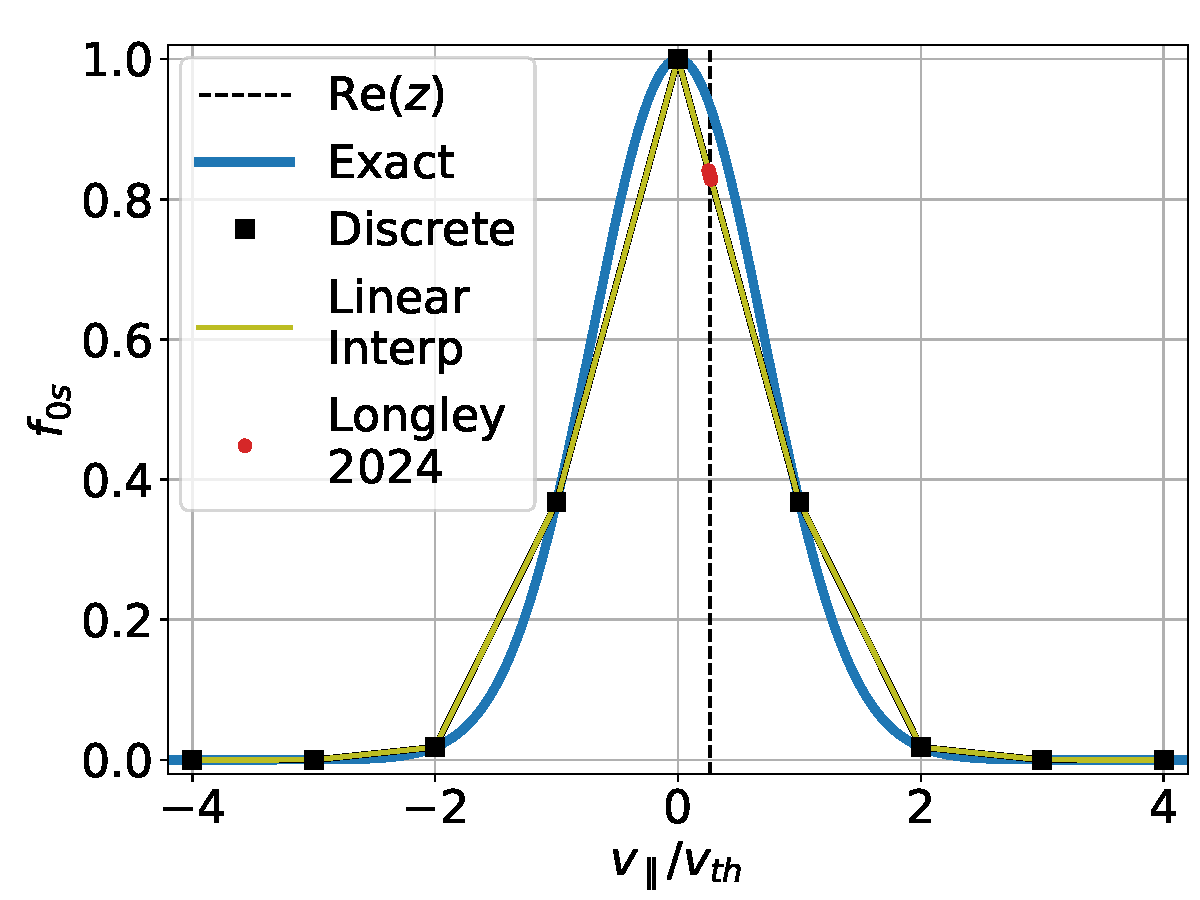
\includegraphics[width=.7\linewidth]{explain.pdf}
	\caption{An example of the representation of a normalized Maxwellian distribution (blue line) with 
	known discrete values (black squares) using either a linear interpolation (green lines)
	or a refined mesh about the pole (red dots) \citep{longley2024}.
	The vertical dashed line represents the real component of the pole, which is defined as $z=\pi/12-10^{-3}i$.}
	\label{f:explainIntegrationMethod}
\end{figure}

Since this method only chooses a finite number of points and can only ever be as good as the interpolation scheme, 
the thought was to instead attempt to get an infinite number of points, i.e., a continuous representation.
Since the adaptive mesh is based on linear interpolation, why not just represent the entire distribution function as a set of 
linear piecewise functions in the parallel direction, as shown by the orange lines.
This gives a continuous representation of the distribution function with each line segment of the interpolated
distribution function described as a linear equation of the form
\begin{equation}
	f_{0s,j} (v_\perp, v_\parallel) = a_j(v_\perp) v_\parallel + b_j (v_\perp),
	\label{eq:fLinear}
\end{equation}
where $a_j$ and $b_j$ are polynomial coefficients calculated using
\begin{align}
	a_j(v_\perp) = \frac{f_{0s}(v_\perp, v_{\parallel,i+1}) - f_{0s}(v_\perp, v_{\parallel,i})}{v_{\parallel,j+1}-v_{\parallel,j}}
	\label{eq:aCoeff} \\
	b_j(v_\perp) = f_{0s}(v_\perp, v_{\parallel,j}) - a_j(v_\perp) v_{\parallel,j}.
	\label{eq:bCoeff}
\end{align}
These are just the standard formulas for calculating linear interpolation coeffients. 
Note that the distribution function is an azimuthally symmetric function of $v_\perp$ and $v_\parallel$.
In our case, we only need to do the linear interpolation in the parallel direction.
Therefore, the coefficients $a_j$ and $b_j$ are functions of $v_\perp$.

% Rethink some of the terminology. It could be improved with all the p's everywhere meaning subtly different things
With this discrete representation, we can obtain the analytic indefinite integrals by substituting Eq.~\ref{eq:fLinear} into Eqs.~\ref{eq:p1}-\ref{eq:p2} yielding
\begin{equation}
	p_1^j (v_\perp, v_\parallel) = \int \frac{f_{0s,j}(v_\parallel,v_\perp)}{v_\parallel - z} dv_\parallel = 
	a_j(v_\perp) \big(v_\parallel-z\big) + \big[ a_j(v_\perp) z + b_j(v_\perp) ] \ln \big( v_\parallel - z \big)
	\label{eq:p1j}
\end{equation}
\begin{equation}
	p_*^j (v_\perp, v_\parallel) =\int \frac{f_{0s,j}(v_\parallel,v_\perp)}{(v_\parallel - z)(v_\parallel - z^*)} dv_\parallel = 
	- \frac{i \Big( \big[ a_j(v_\perp)z + b_j(v_\perp)\big] \ln \big[ v_\parallel-z \big] - 
		\big[ a_j(v_\perp)z^* + b_j(v_\perp)\big] \ln \big[ v_\parallel-z^* \big] 
		\Big)  }{2 \im(z)},
	\label{eq:pstarj}
\end{equation}
\begin{equation}
	p_2^j (v_\perp, v_\parallel) =\int \frac{f_{0s,j}(v_\parallel,v_\perp)}{(v_\parallel - z)^2} dv_\parallel = 
	\frac{-a_j(v_\perp)z - b_j(v_\perp)}{v_\parallel - z} + a_j(v_\perp) \ln\big(v_\parallel-z\big)
	\label{eq:p2j}
\end{equation}
where $p_1^j(v_\perp)$, $p_*^j(v_\perp)$, and $p_2^j(v_\perp)$ are the indefinite integrals corresponding to 
Eqs.~\ref{eq:p1}-\ref{eq:p2}, respectively, for element $j$.
We can obtain the full integration from $-\infty$ to $\infty$ (which is realistically $-v_{\parallel,\max}$ to $v_{\parallel,\max}$)
\begin{equation}
	p(v_\perp) = \sum_j p^j(v_\perp, v_{\parallel,j+1}) - p^j(v_\perp, v_{\parallel,j}),
	\label{eq:finalPoleIntegral}
\end{equation}
where $p$ is a placeholder for the specific pole integral being carried out from Eqs.~\ref{eq:p1j} to \ref{eq:p2j}.

% Maybe we say somewhere that the second order pole is the most difficult to get right because of it being an even function about the pole (no terms to cancel).

We will test this pole integration method with the normalized Maxwellian distribution function from Eq.~\ref{eq:norm_maxwellian} with the known exact solutions from Eqs.~\ref{eq:p1Exact}-\ref{eq:p2Exact}.
The pole is chosen to be at $z=\pi/12 - i \gamma$ where $\gamma=(\nu/k_\parallel)/v_{th}$ (see Eq.~\ref{eq:z}) is varied logarithmically from $10^{-6}$ to $10^{0}$.
Note that the real part of $z$ is chosen specifically to be irrational such that it will always be in between the discrete points. 
This provides the best case scenario for our method.

Figs.~\ref{f:poleIntegrateError0}-\ref{f:poleIntegrateError-5} show how the linear pole integration from Eq.~\ref{eq:finalPoleIntegral} (red x's) compares with the exact solution from Eqs.~\ref{eq:p1Exact}-\ref{eq:p2Exact} (black line), a simple trapezoidal integration (orange dots), and the pole refinement technique \citep{longley2024} (blue circles) for varying discrete velocity mesh resolutions varying from $\Delta v_\parallel/v_{th}=10^0$ to $\Delta v_\parallel/v_{th}=10^{-5}$.
We show the real (top) and imaginary (bottom) solutions for each of the three poles from Eqs.~\ref{eq:p1}-\ref{eq:p2}.
The $x$-axis of all of these plots is $\gamma$. 
Since the real part of the pole is constant at 0.25, the $\gamma$ can be seen as the distance of the pole from the real axis.
As $\gamma$ approaches $\infty$, or as we move to the right in Figs.~\ref{f:poleIntegrateError0}-\ref{f:poleIntegrateError-5}, the pole moves further away from the real axis.
The further the pole is from the real axis, the less it impacts the final integration result resulting in an easier calculation.
As $\gamma$ approaches 0, or as we move to the left in Figs.~\ref{f:poleIntegrateError0}-\ref{f:poleIntegrateError-5}, the pole approaches the real axis.
The closer the pole is to the real axis, the more difficult the calculations are.
Therefore, the solutions for all of the integration methods are expected to be more correct towards the right and have more error towards the left.

Fig.~\ref{f:poleIntegrateError0} has the coarsest mesh and presents why this linear interpolation method is so powerful.
The velocity mesh and the discrete distribution function correspond exactly to the example in Fig.~\ref{f:explainIntegrationMethod}.
As would be expected for representing a Maxwellian distribution using only 9 points, trapezoidal is only correct toward the right where the pole is far from the real axis.
The pole refined integration technique is an improvement and is generally more correct for more values of $\gamma$.
The linear interpolation integration method shows significant improvement over all of the other methods and provides generally correct asymptotic behavor as $\gamma$ approaches 0 that the other methods do not.
Thus, for even a very coarse mesh of only 9 points, our technique is significantly better than previously used methods.


A very nice result for all of the methods is that the imaginary component of the double pole at $z$ and $z^*$ (Eq.~\ref{eq:pstar}) should be exactly 0 (Eq.~\ref{eq:pstarExact}).
Every integration method captures this behavior.
% Dunno what else to say here, but, just wanted to explicitly point this out somewhere


As we increase the mesh resolution to have $\Delta v_\parallel/v_{th}=10^{-1}$, each of the methods generally improve.
This will be the case for each increase in resolution.
The pole refined, linear interpolation, and trapezoidal methods fully capture the real part of the first order pole. 
The linear interpolation method fully captures the real part of the double pole and the imaginary part of the second order pole.
Furthermore, the linear interpolation method almost exactly captures the real part of the second order pole.


At a resolution of $\Delta v_\parallel/v_{th}=10^{-2}$, the linear interpolation appears to fully capture the real part of the second order pole.
At this resolution, the linear interpolation method has now fully captured all of the calculations. 
Note that in testing this for the full spectrum calculations, we found that $\Delta v_\parallel/v_{th}=10^{-2.3}$ provided sufficient parallel velocity resolution to reach a converged solution. 
This will likely have to modified depending on the structure of the distribution function.

The other methods just provide general improvements for this increased resolution. 
This is the case for $\Delta v_\parallel/v_{th}=10^{-3}$ as well.
At $\Delta v_\parallel/v_{th}=10^{-4}$, the pole refined method fully captures everything but the real part of the second order pole.
Even at the finest resolution tested at $\Delta v_\parallel/v_{th}=10^{-5}$, the real part of the second order pole is never fully captured.
Interestingly, the trapezoidal integration at this resolution actually provides better results than the pole refined method for certain $\gamma$ (which also happen to be around realistic ionospheric and radar values).
Nonetheless, Figs.~\ref{f:poleIntegrateError0}-\ref{f:poleIntegrateError-5} show the superiority of the linear interpolation method versus the other methods.

% I should add Gaussian quadrature as another integration method here?
\begin{figure}[!htb]
	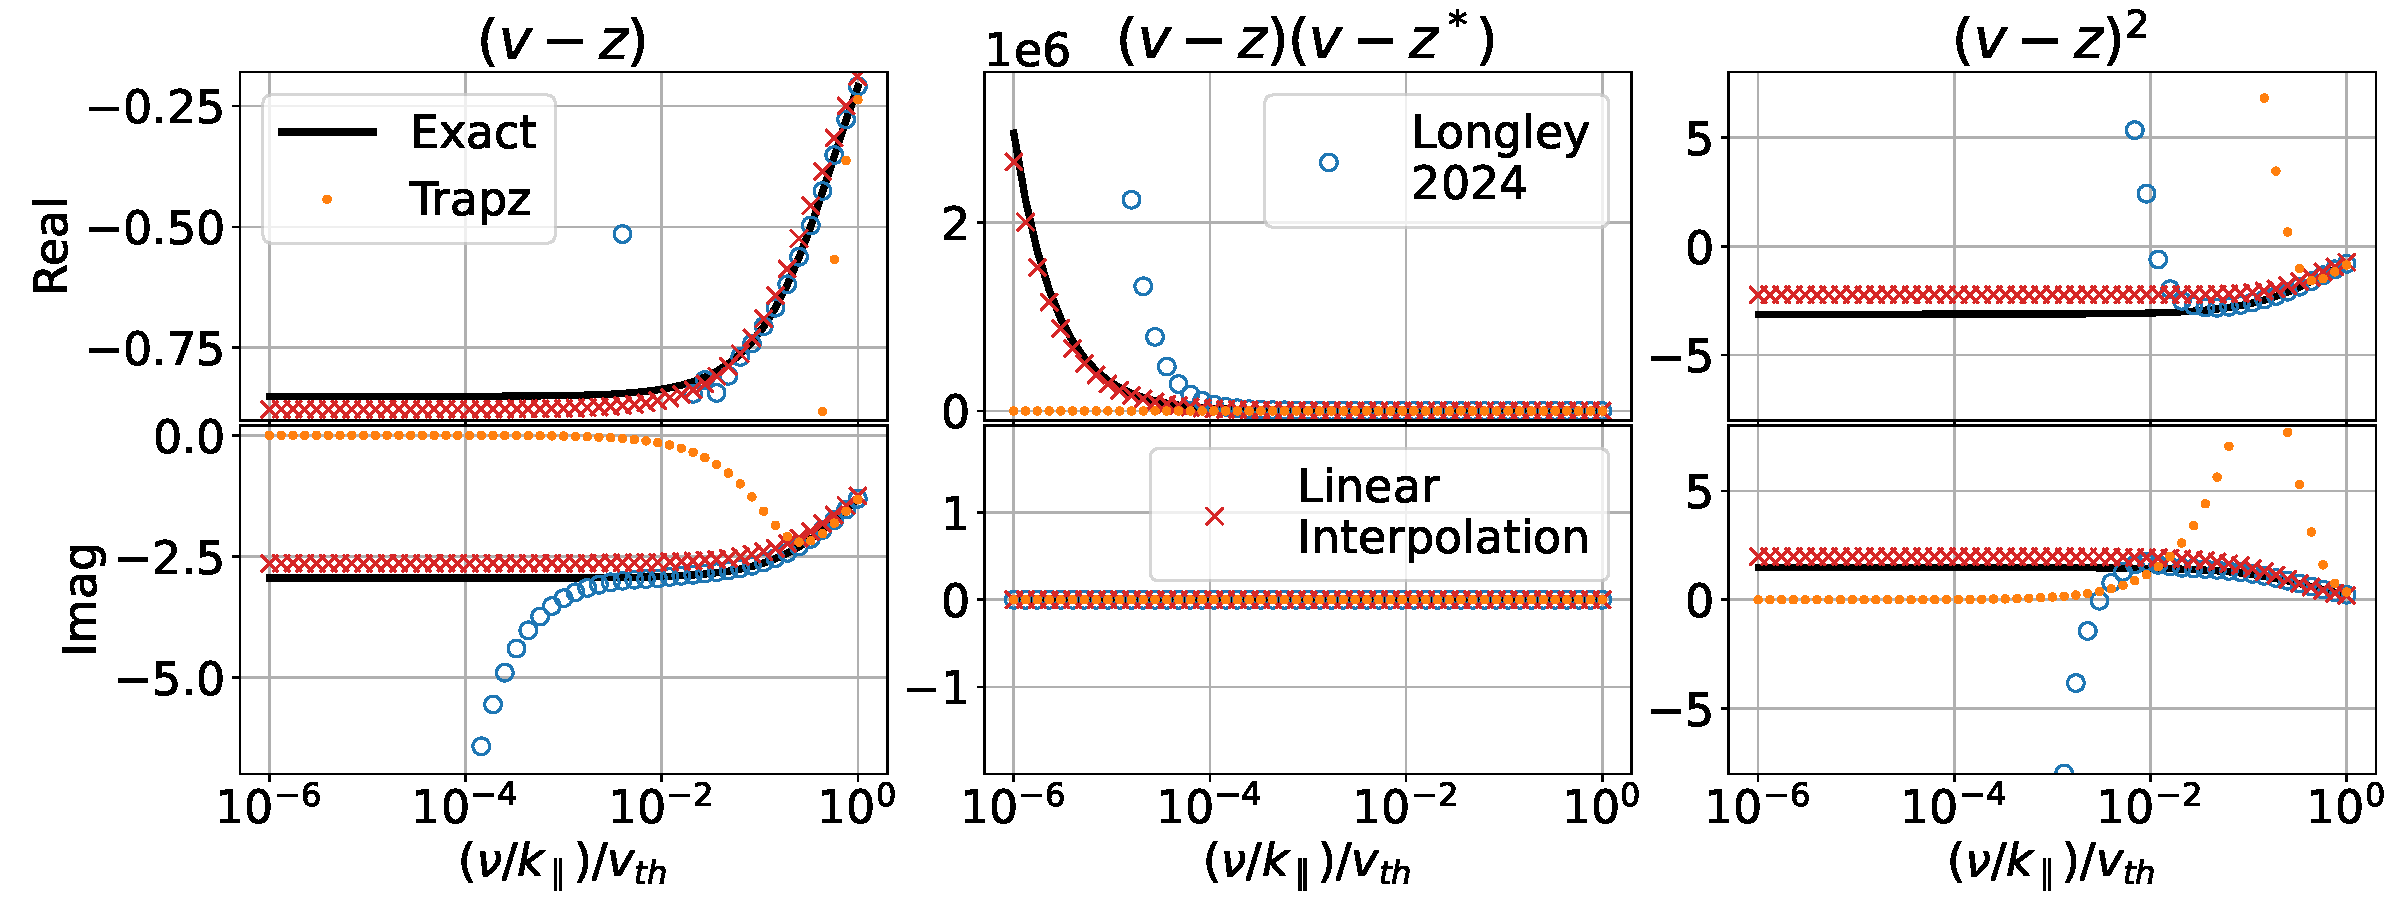
\includegraphics[width=\linewidth]{poleIntegrate_error_0.pdf}
	\caption{Comparison of error between exact solution from Eqs.~\ref{eq:p1Exact}-\ref{eq:p2Exact} (black line),
		trapezoidal integration (orange dots),
		pole refined method from \cite{longley2024} (blue circles),
		and our linear interpolation method from Eqs.~\ref{eq:finalPoleIntegral} (red x's).
		Each column corresponds to the solution for a different pole (Eqs.~\ref{eq:p1}-\ref{eq:p2}, respectively)
		with the real and imaginary parts on the top and bottom panels, respectively.
		The pole is $z=\pi/12-i\gamma$.
		The original mesh resolution is $\Delta v_\parallel/v_{th}=10^0$.}
	\label{f:poleIntegrateError0}
\end{figure}

\begin{figure}[!htb]
	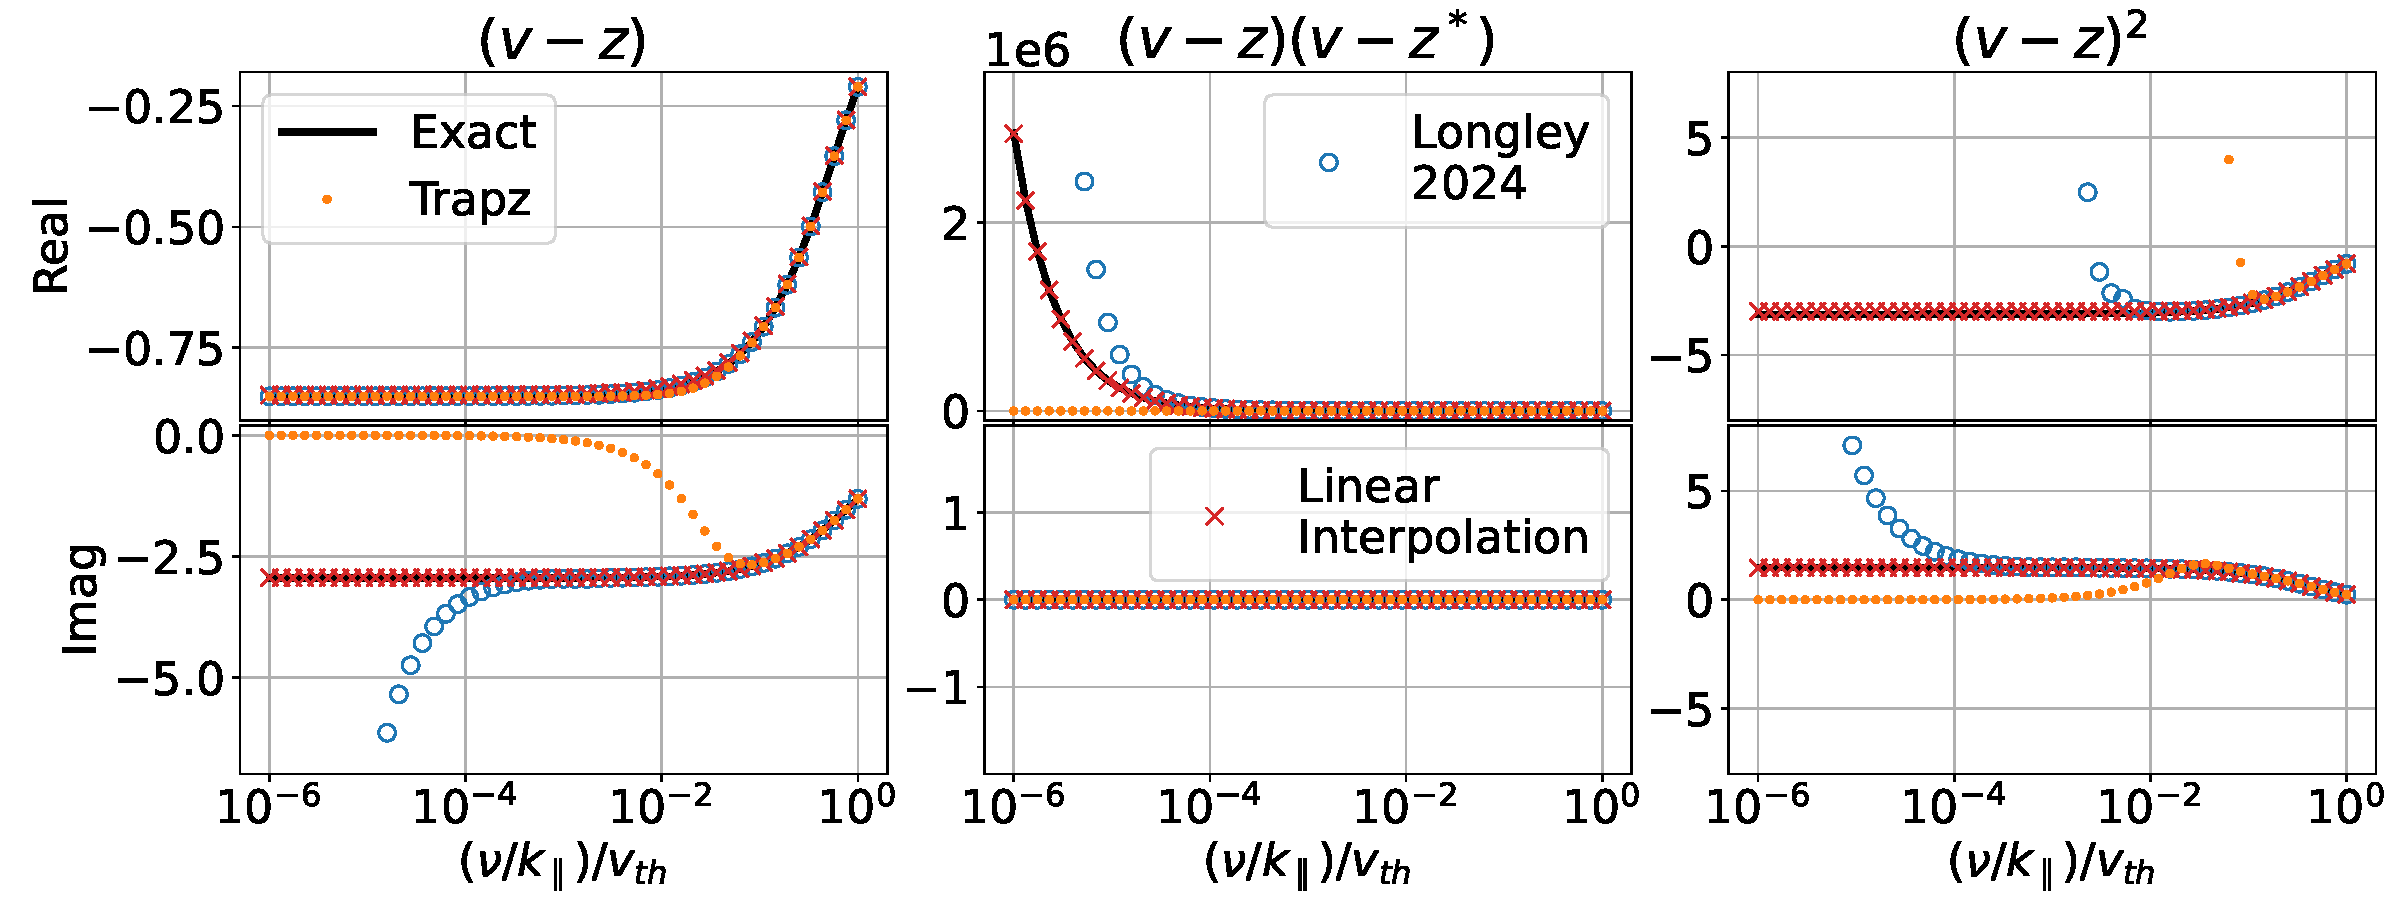
\includegraphics[width=\linewidth]{poleIntegrate_error_-1.pdf}
	\caption{Same as Fig.~\ref{f:poleIntegrateError0} but with $\Delta v_\parallel/v_{th}=10^{-1}$.}
	\label{f:poleIntegrateError-1}
\end{figure}

\begin{figure}[!htb]
	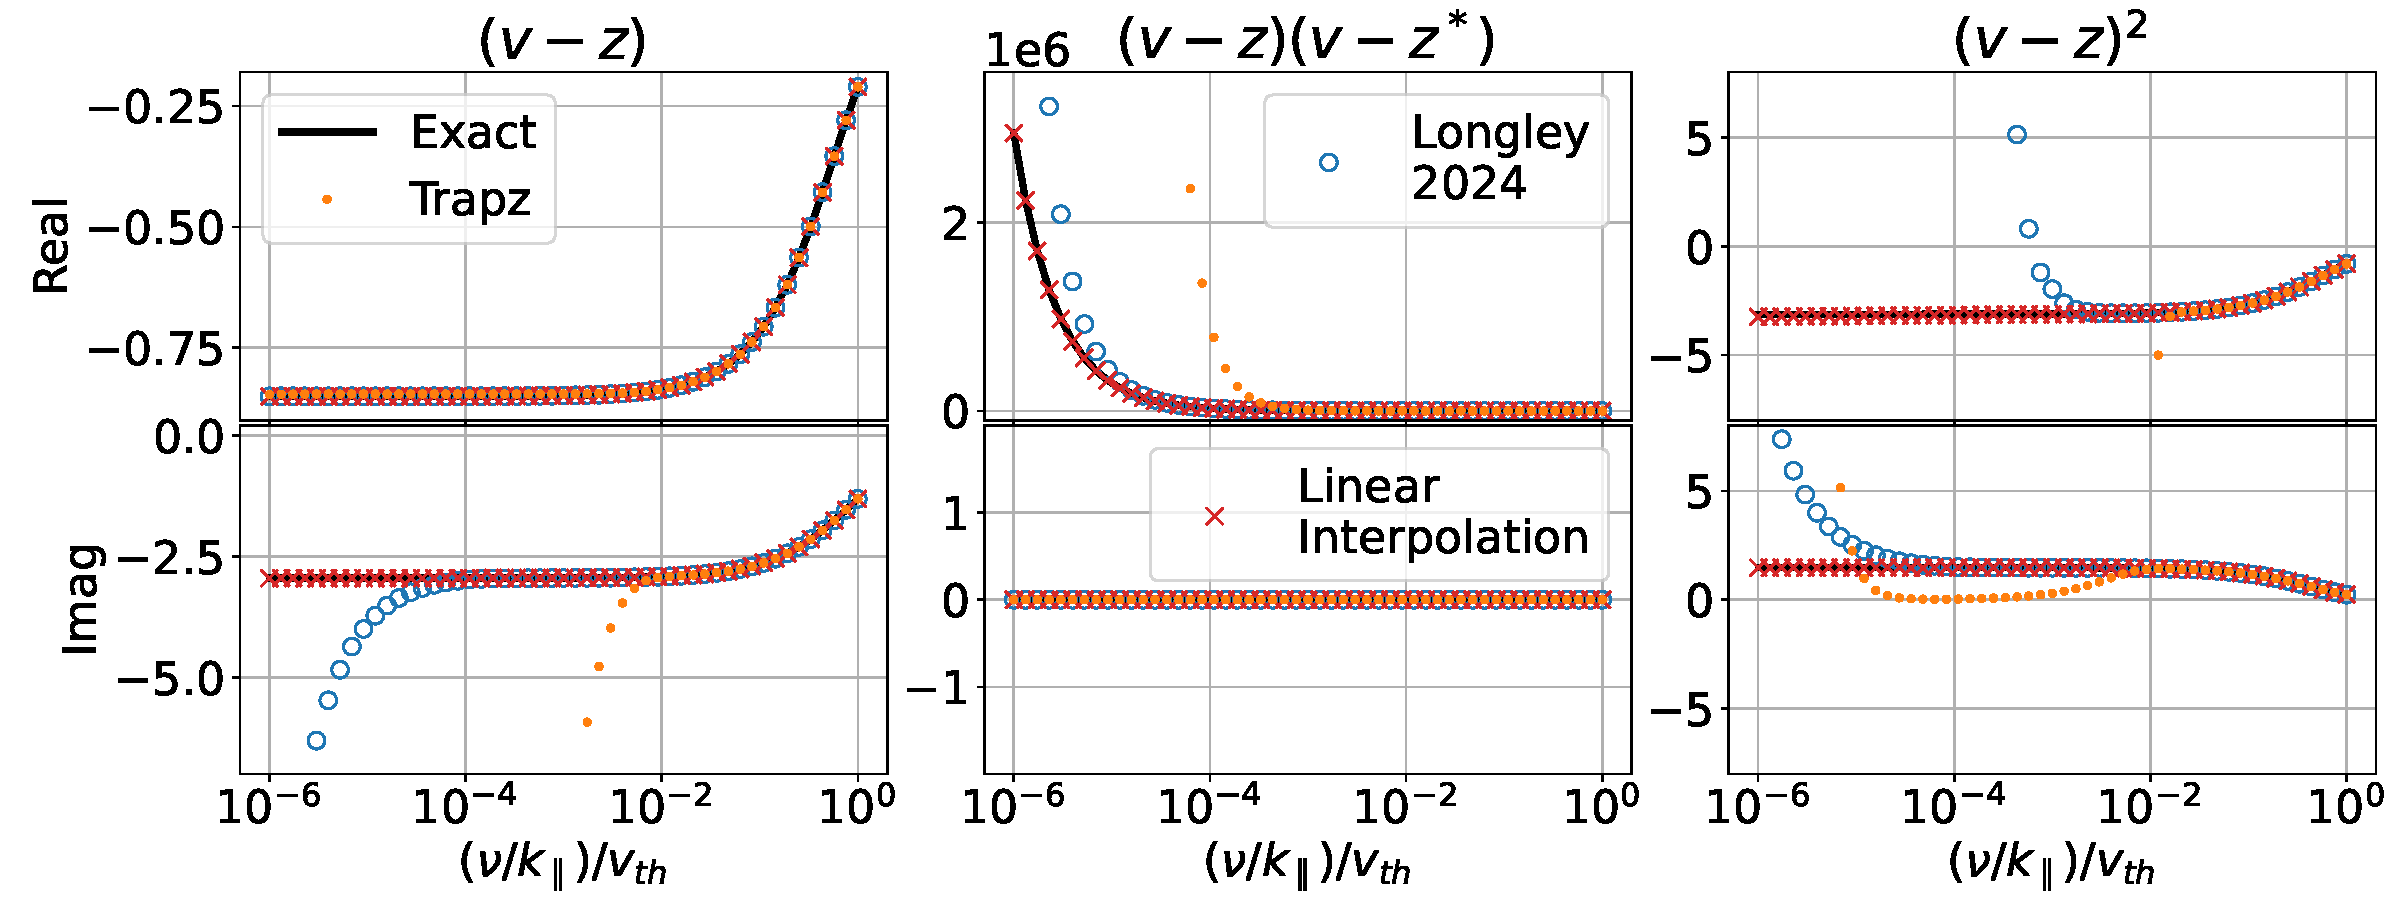
\includegraphics[width=\linewidth]{poleIntegrate_error_-2.pdf}
	\caption{Same as Fig.~\ref{f:poleIntegrateError0} but with $\Delta v_\parallel/v_{th}=10^{-2}$.}
	\label{f:poleIntegrateError-2}
\end{figure}

\begin{figure}[!htb]
	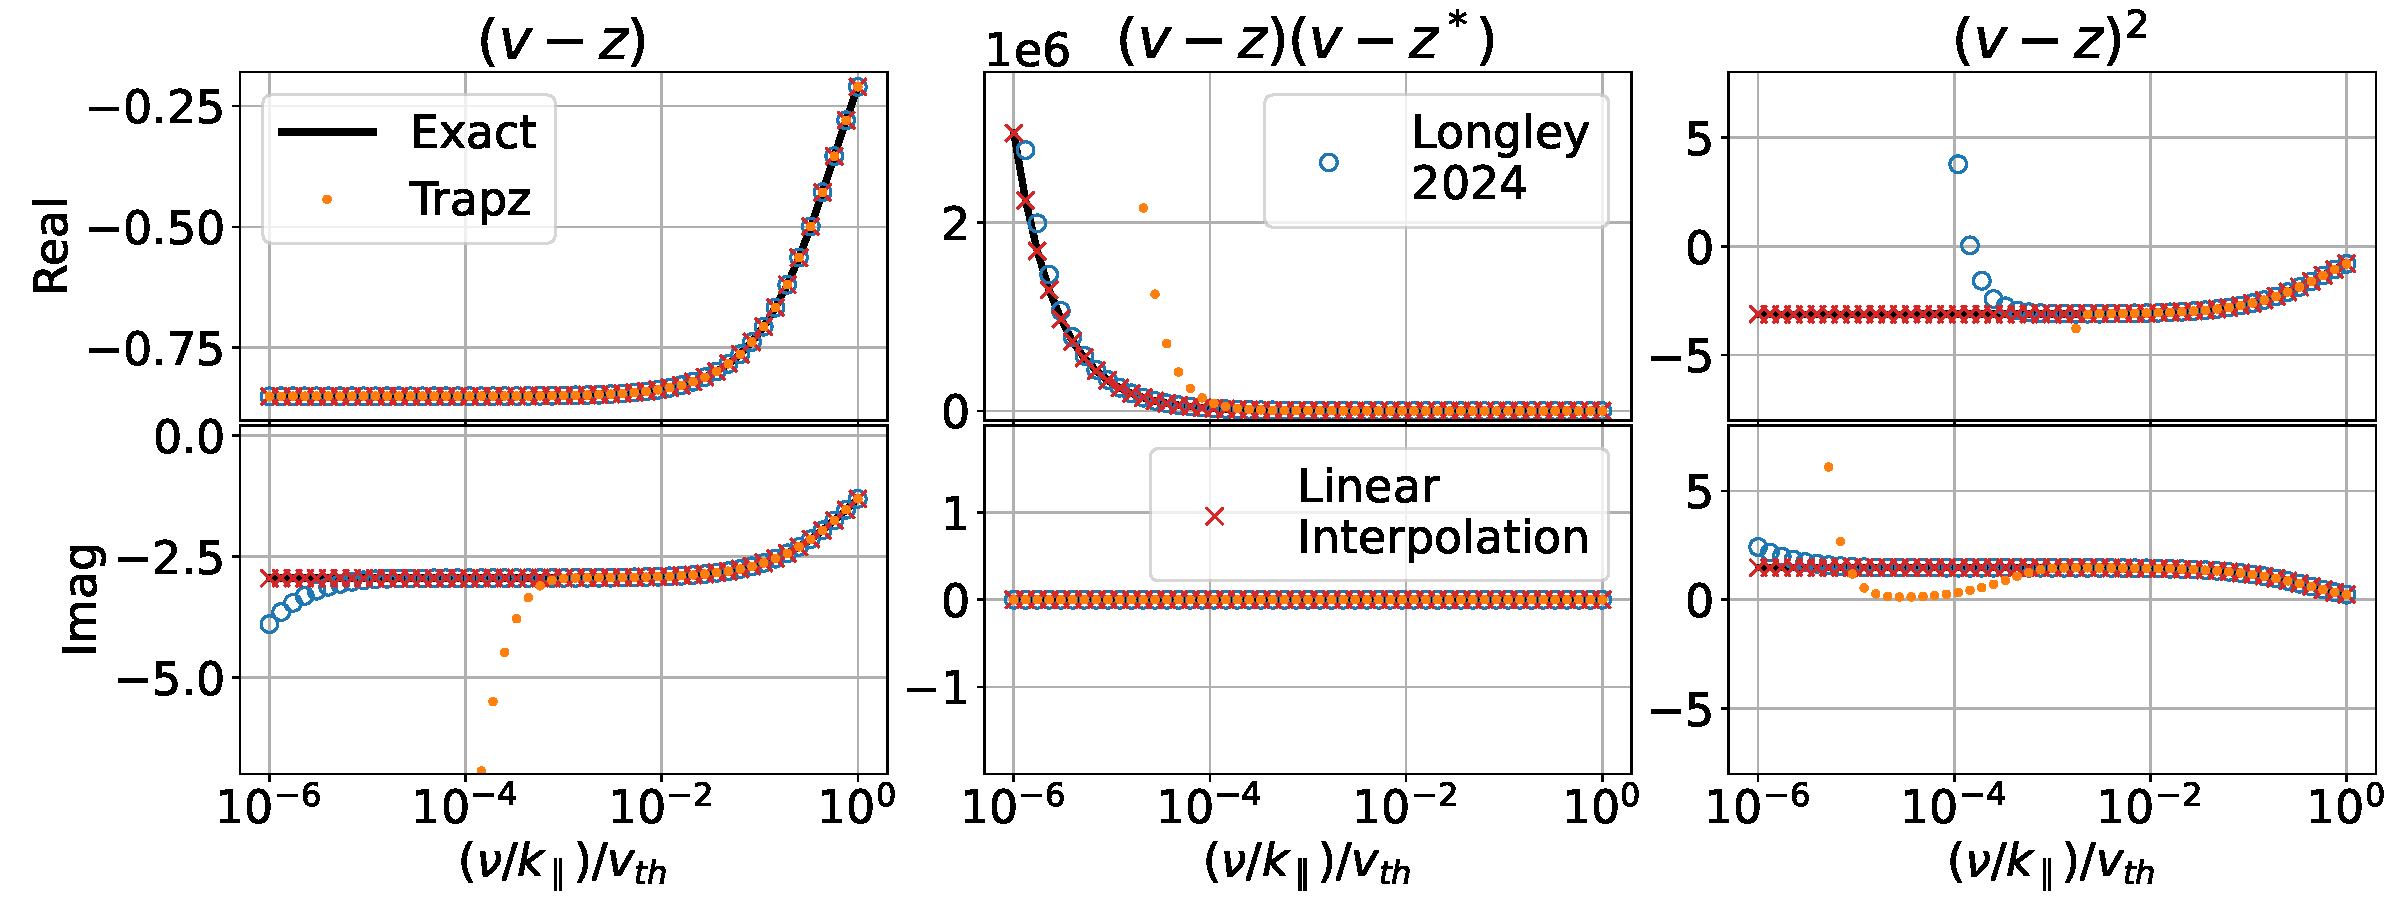
\includegraphics[width=\linewidth]{poleIntegrate_error_-3.pdf}
	\caption{Same as Fig.~\ref{f:poleIntegrateError0} but with $\Delta v_\parallel/v_{th}=10^{-3}$.}
	\label{f:poleIntegrateError-3}
\end{figure}

\begin{figure}[!htb]
	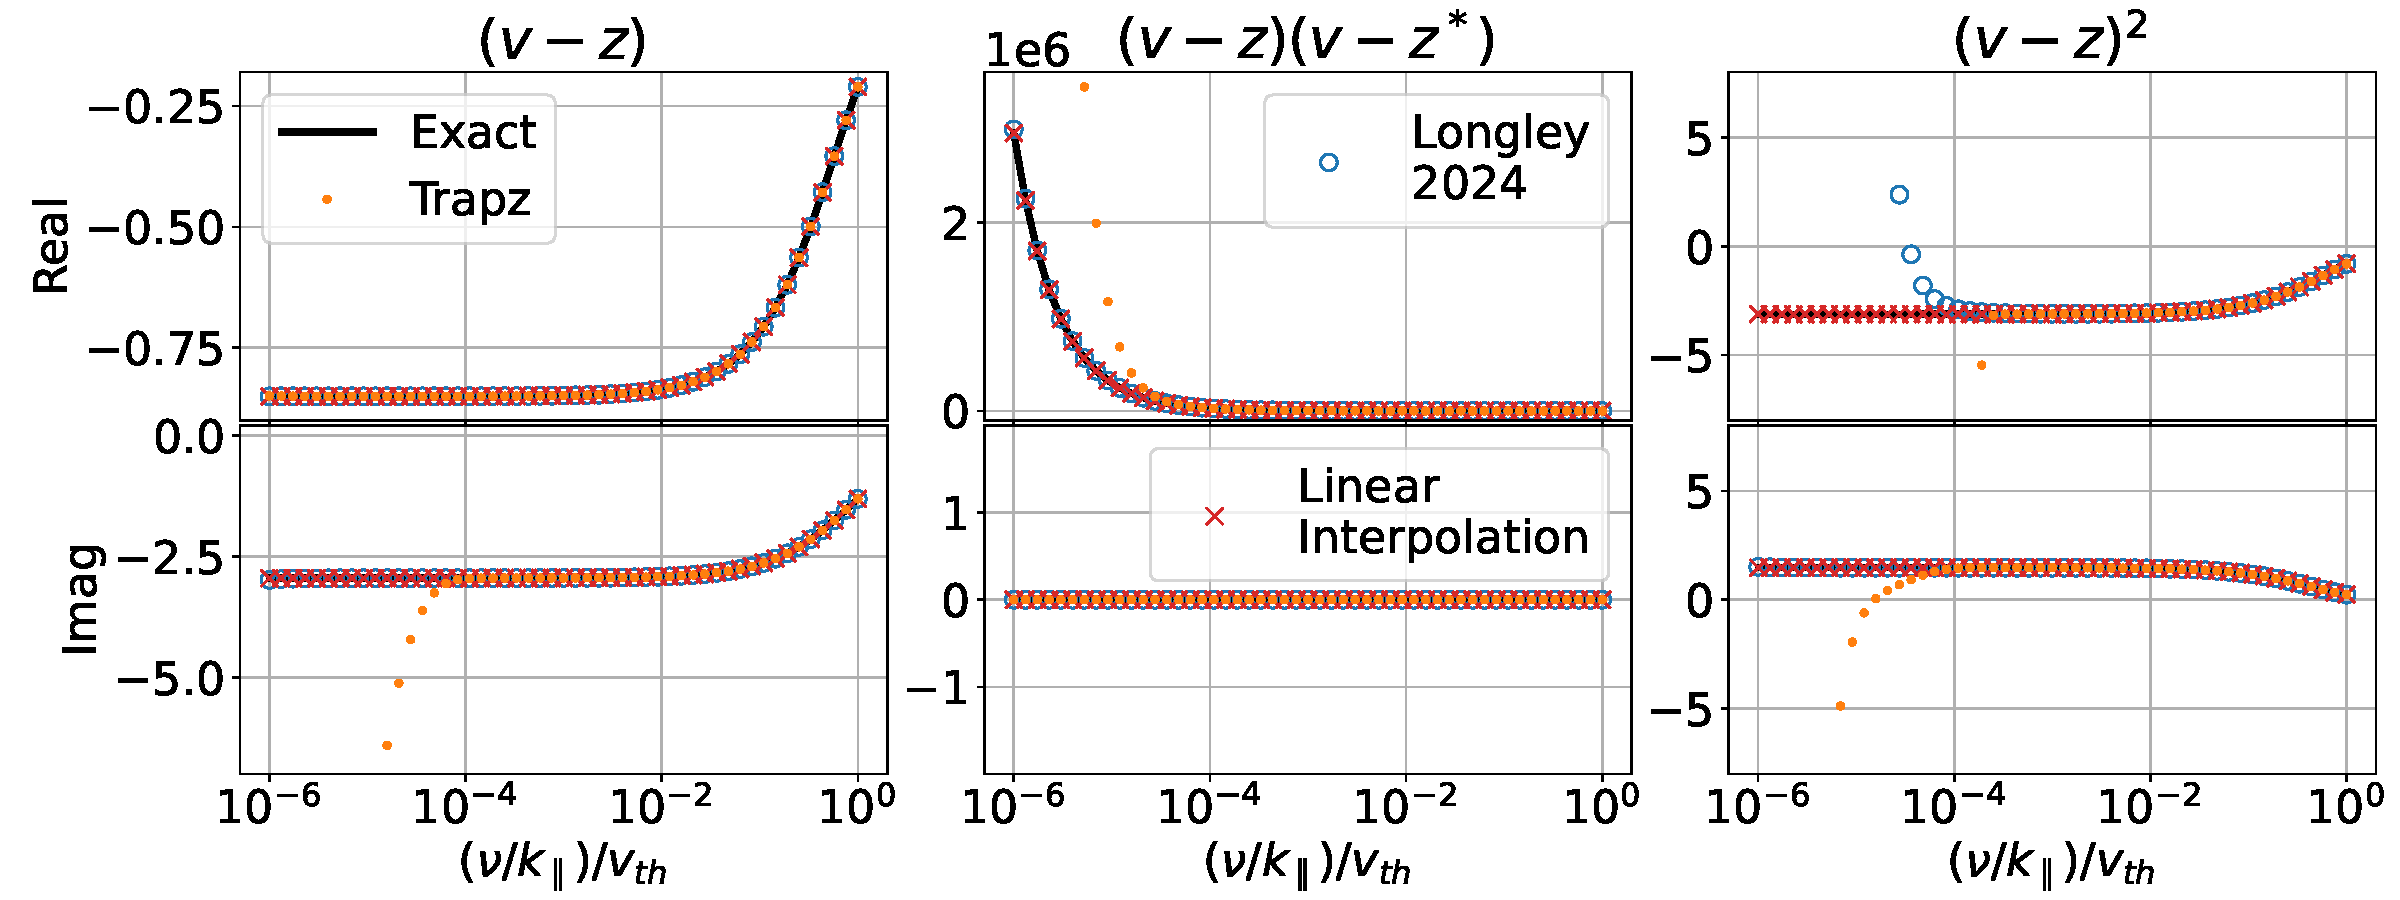
\includegraphics[width=\linewidth]{poleIntegrate_error_-4.pdf}
	\caption{Same as Fig.~\ref{f:poleIntegrateError0} but with $\Delta v_\parallel/v_{th}=10^{-4}$.}
	\label{f:poleIntegrateError-4}
\end{figure}

\begin{figure}[!htb]
	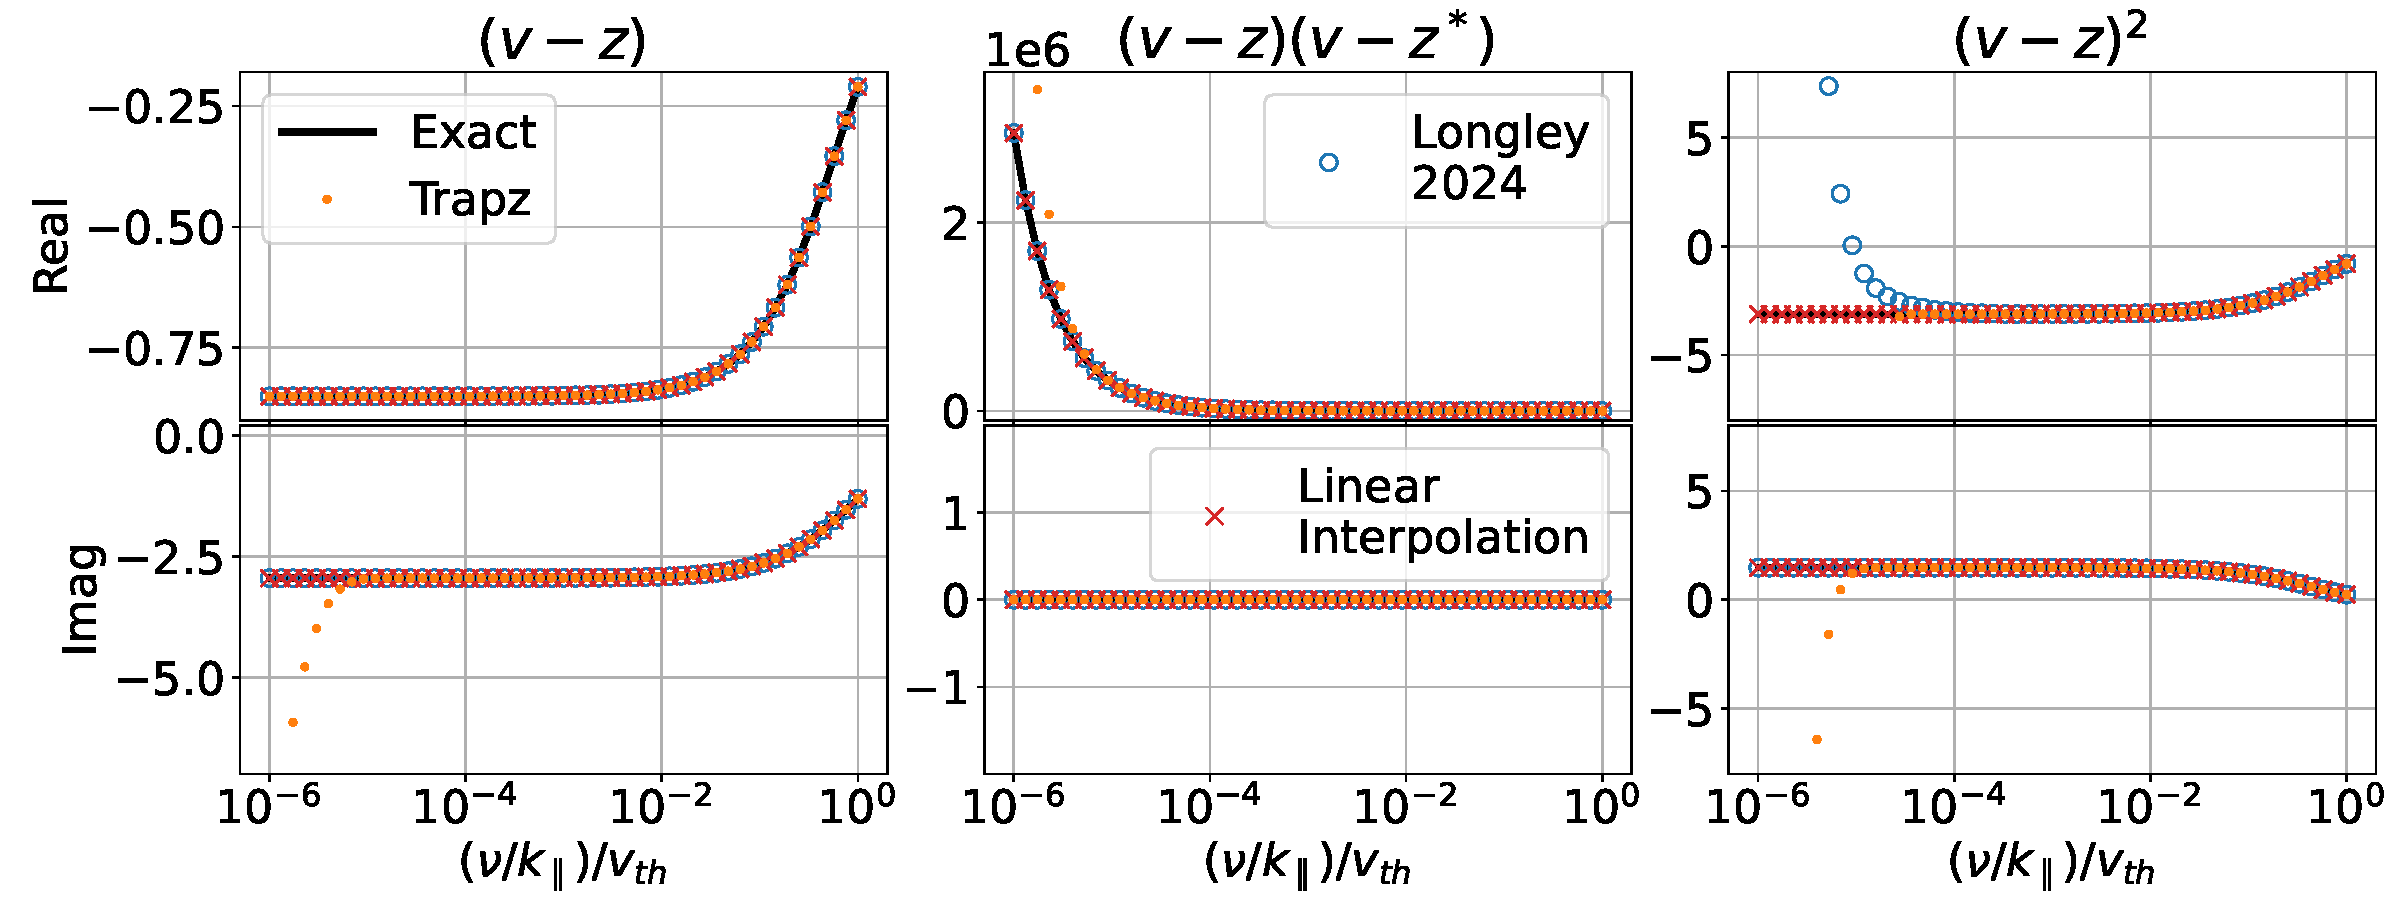
\includegraphics[width=\linewidth]{poleIntegrate_error_-5.pdf}
	\caption{Same as Fig.~\ref{f:poleIntegrateError0} but with $\Delta v_\parallel/v_{th}=10^{-5}$.}
	\label{f:poleIntegrateError-5}
\end{figure}

Now, these are for the best case scenario where the real part of the pole is not in between the discrete points.
In the case where the real part is exactly on a discrete value, what would this look like? 
Figs.~\ref{f:poleIntegrateError0_pole0}-\ref{f:poleIntegrateError-5_pole0} show the same general type of plots as Figs.~\ref{f:poleIntegrateError0}-\ref{f:poleIntegrateError-5} but with the pole at $z=0-i\gamma$.
This will ensure that for every possible resolution, the pole will coincide with a point on the discrete velocity mesh.
We find the same general trends as in the Figs.~\ref{f:poleIntegrateError0}-\ref{f:poleIntegrateError-5}.
The only difference is that our linear interpolation method requires a resolution of $\Delta v_\parallel/v_{th}=10^{-3}$ to converge to the exact solution.
This is likely one of the reasons it requires a mesh of $\Delta v_\parallel/v_{th}=10^{-2.3}$ to reach convergence for the full spectrum calculation.


\begin{figure}[!htb]
	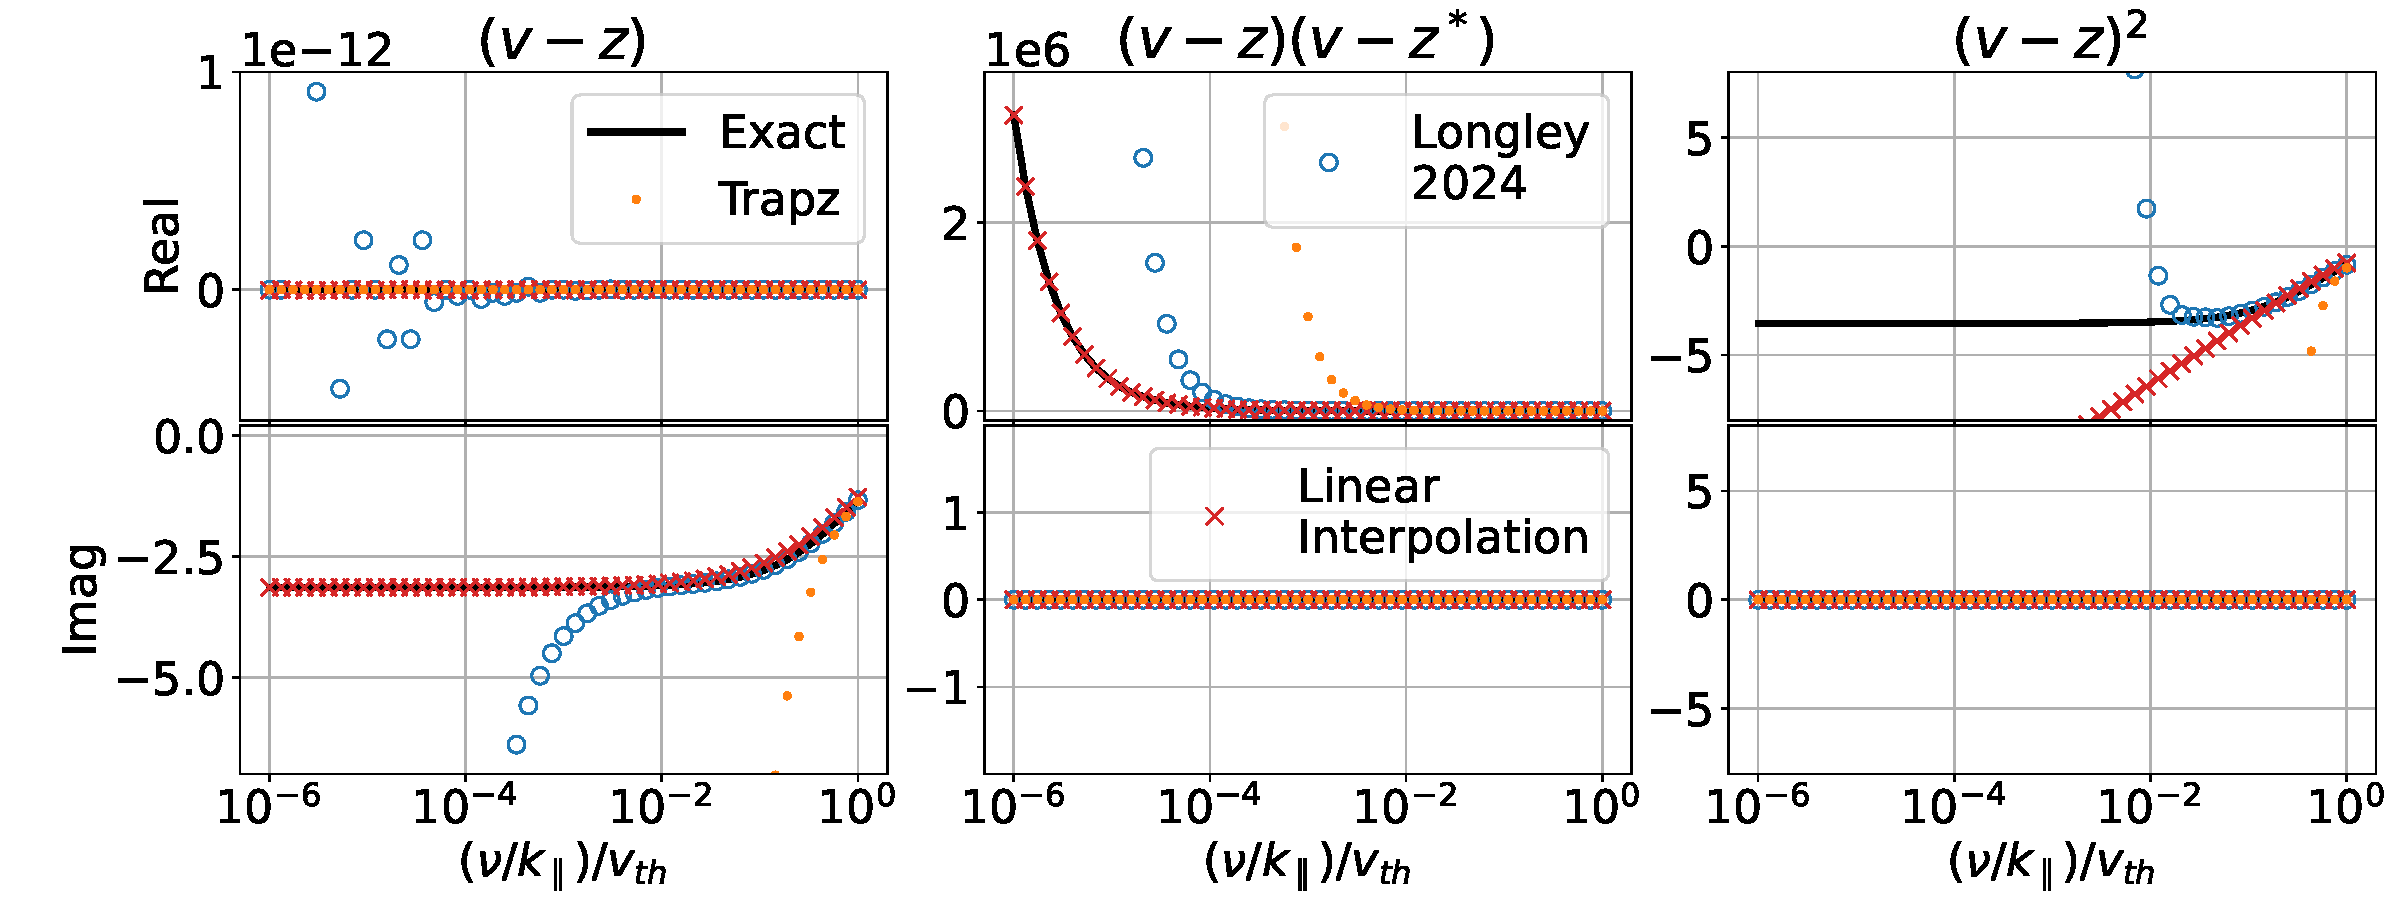
\includegraphics[width=\linewidth]{poleIntegrate_error_pole0_0.pdf}
	\caption{Comparison of error between exact solution from Eqs.~\ref{eq:p1Exact}-\ref{eq:p2Exact} (black line),
		trapezoidal integration (orange dots),
		pole refined method from \cite{longley2024} (blue circles),
		and our linear interpolation method from Eqs.~\ref{eq:finalPoleIntegral} (red x's).
		Each column corresponds to the solution for a different pole (Eqs.~\ref{eq:p1}-\ref{eq:p2}, respectively)
		with the real and imaginary parts on the top and bottom panels, respectively.
		The pole is $z=\pi/12-i\gamma$.
		The original mesh resolution is $\Delta v_\parallel/v_{th}=10^0$.}
	\label{f:poleIntegrateError0_pole0}
\end{figure}

\begin{figure}[!htb]
	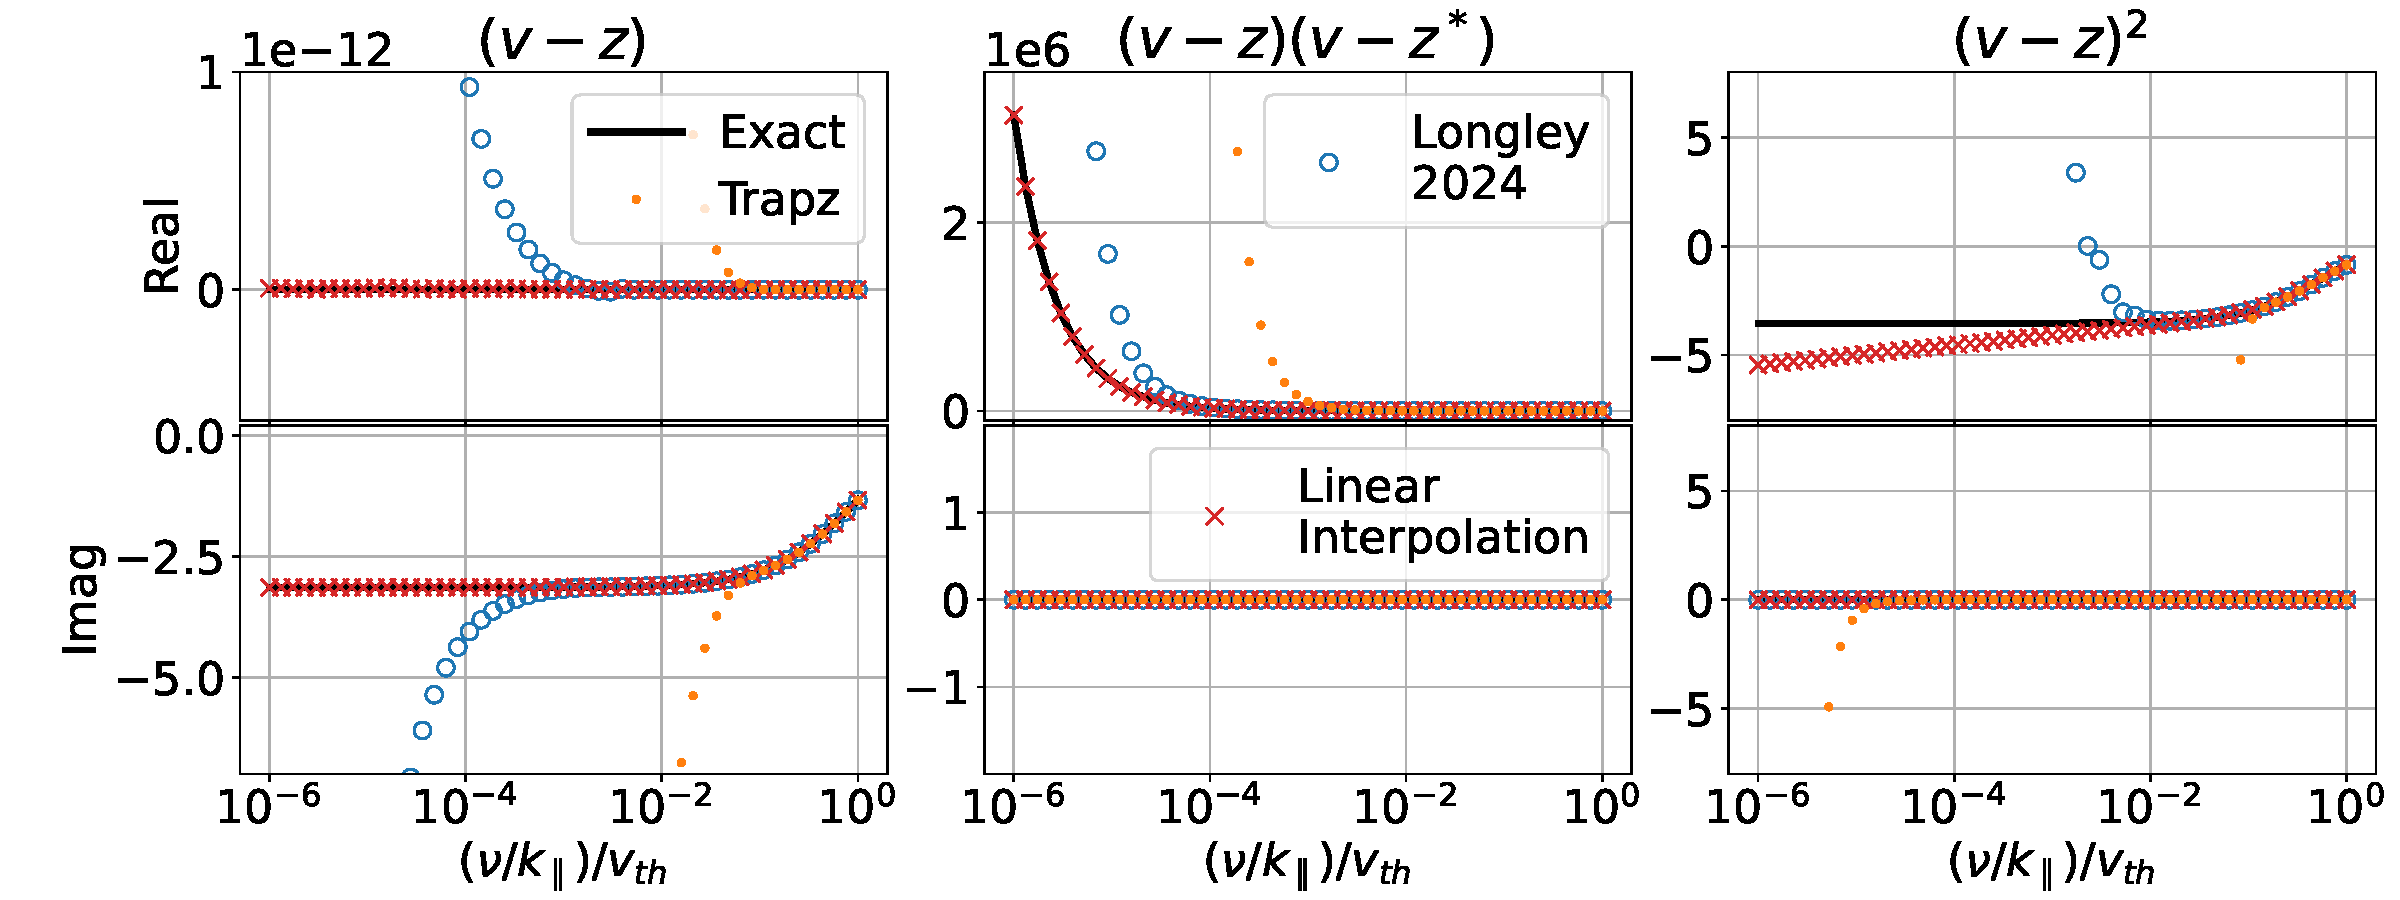
\includegraphics[width=\linewidth]{poleIntegrate_error_pole0_-1.pdf}
	\caption{Same as Fig.~\ref{f:poleIntegrateError0_pole0} but with $\Delta v_\parallel/v_{th}=10^{-1}$.}
	\label{f:poleIntegrateError-1_pole0}
\end{figure}

\begin{figure}[!htb]
	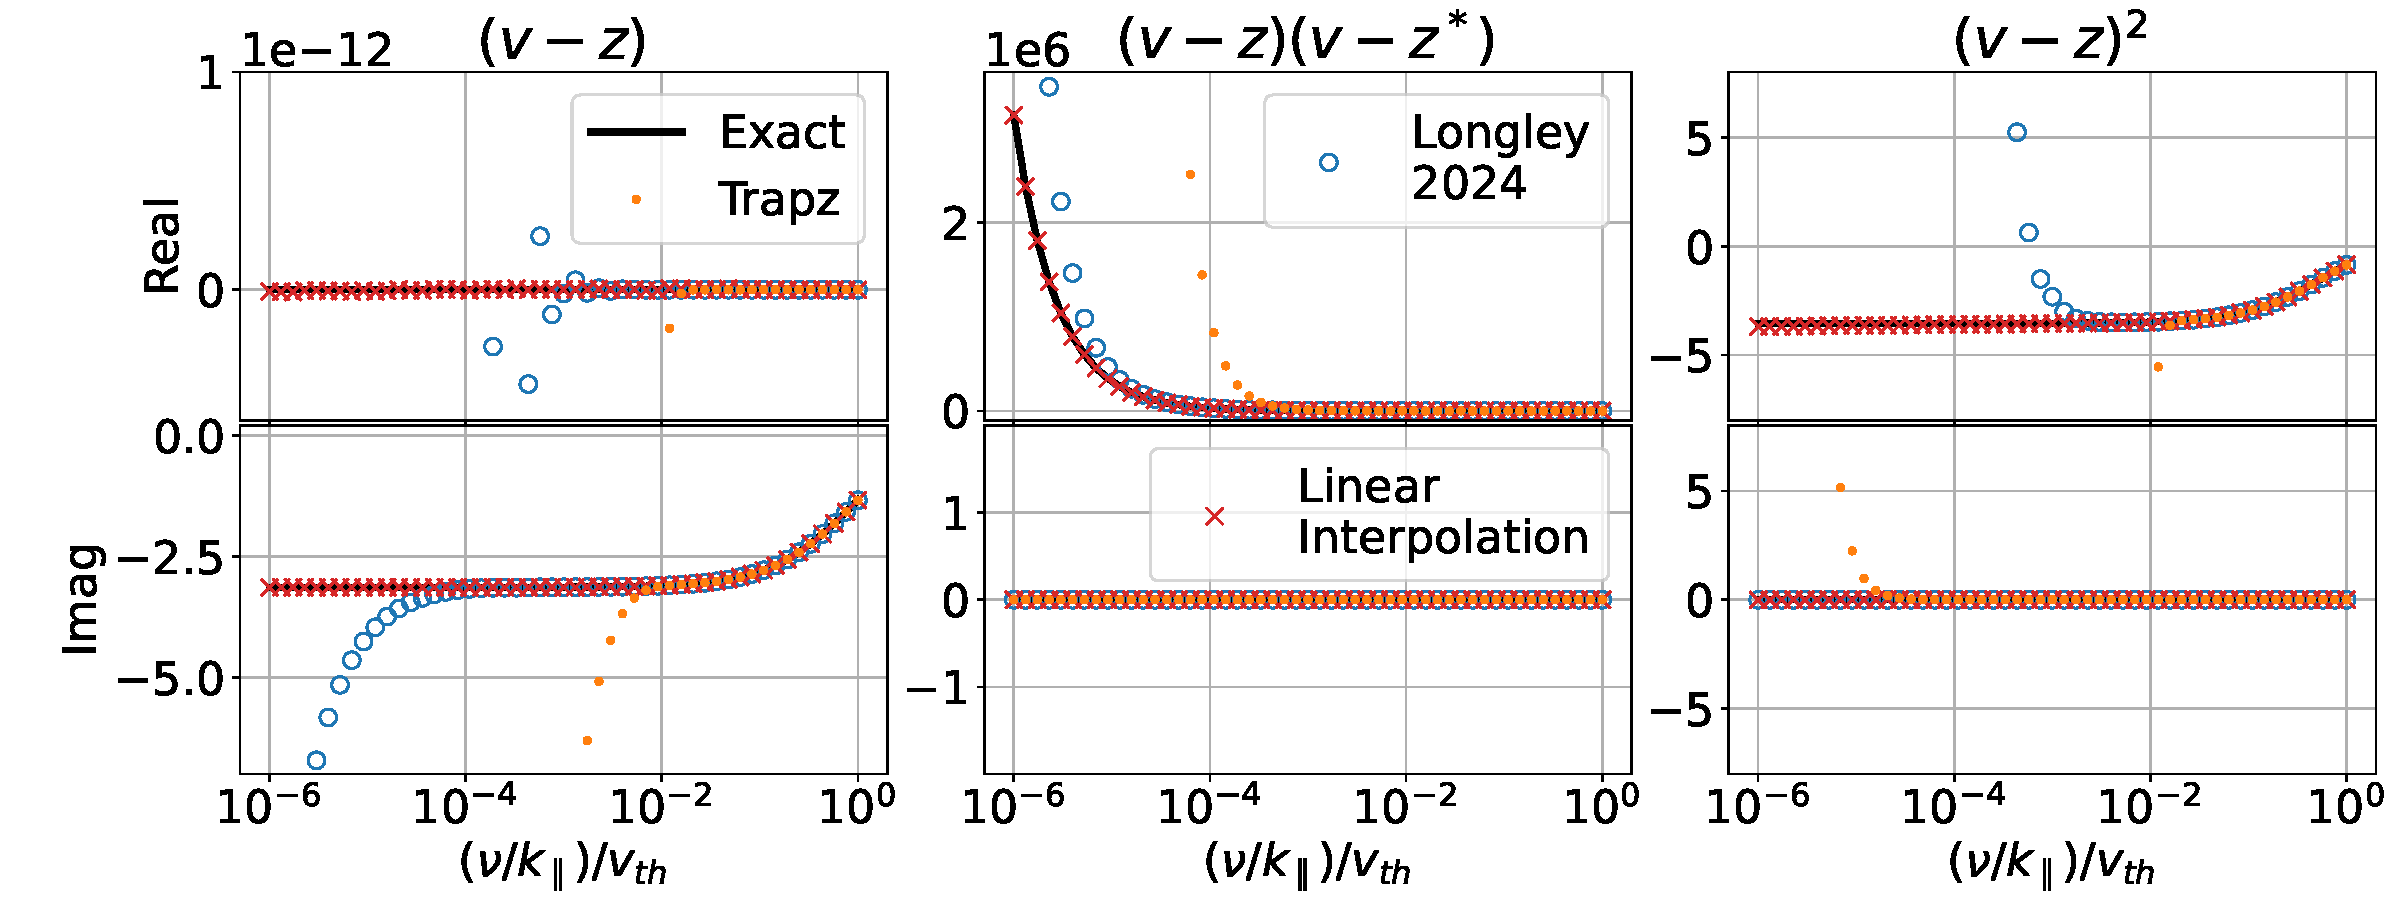
\includegraphics[width=\linewidth]{poleIntegrate_error_pole0_-2.pdf}
	\caption{Same as Fig.~\ref{f:poleIntegrateError0_pole0} but with $\Delta v_\parallel/v_{th}=10^{-2}$.}
	\label{f:poleIntegrateError-2_pole0}
\end{figure}

\begin{figure}[!htb]
	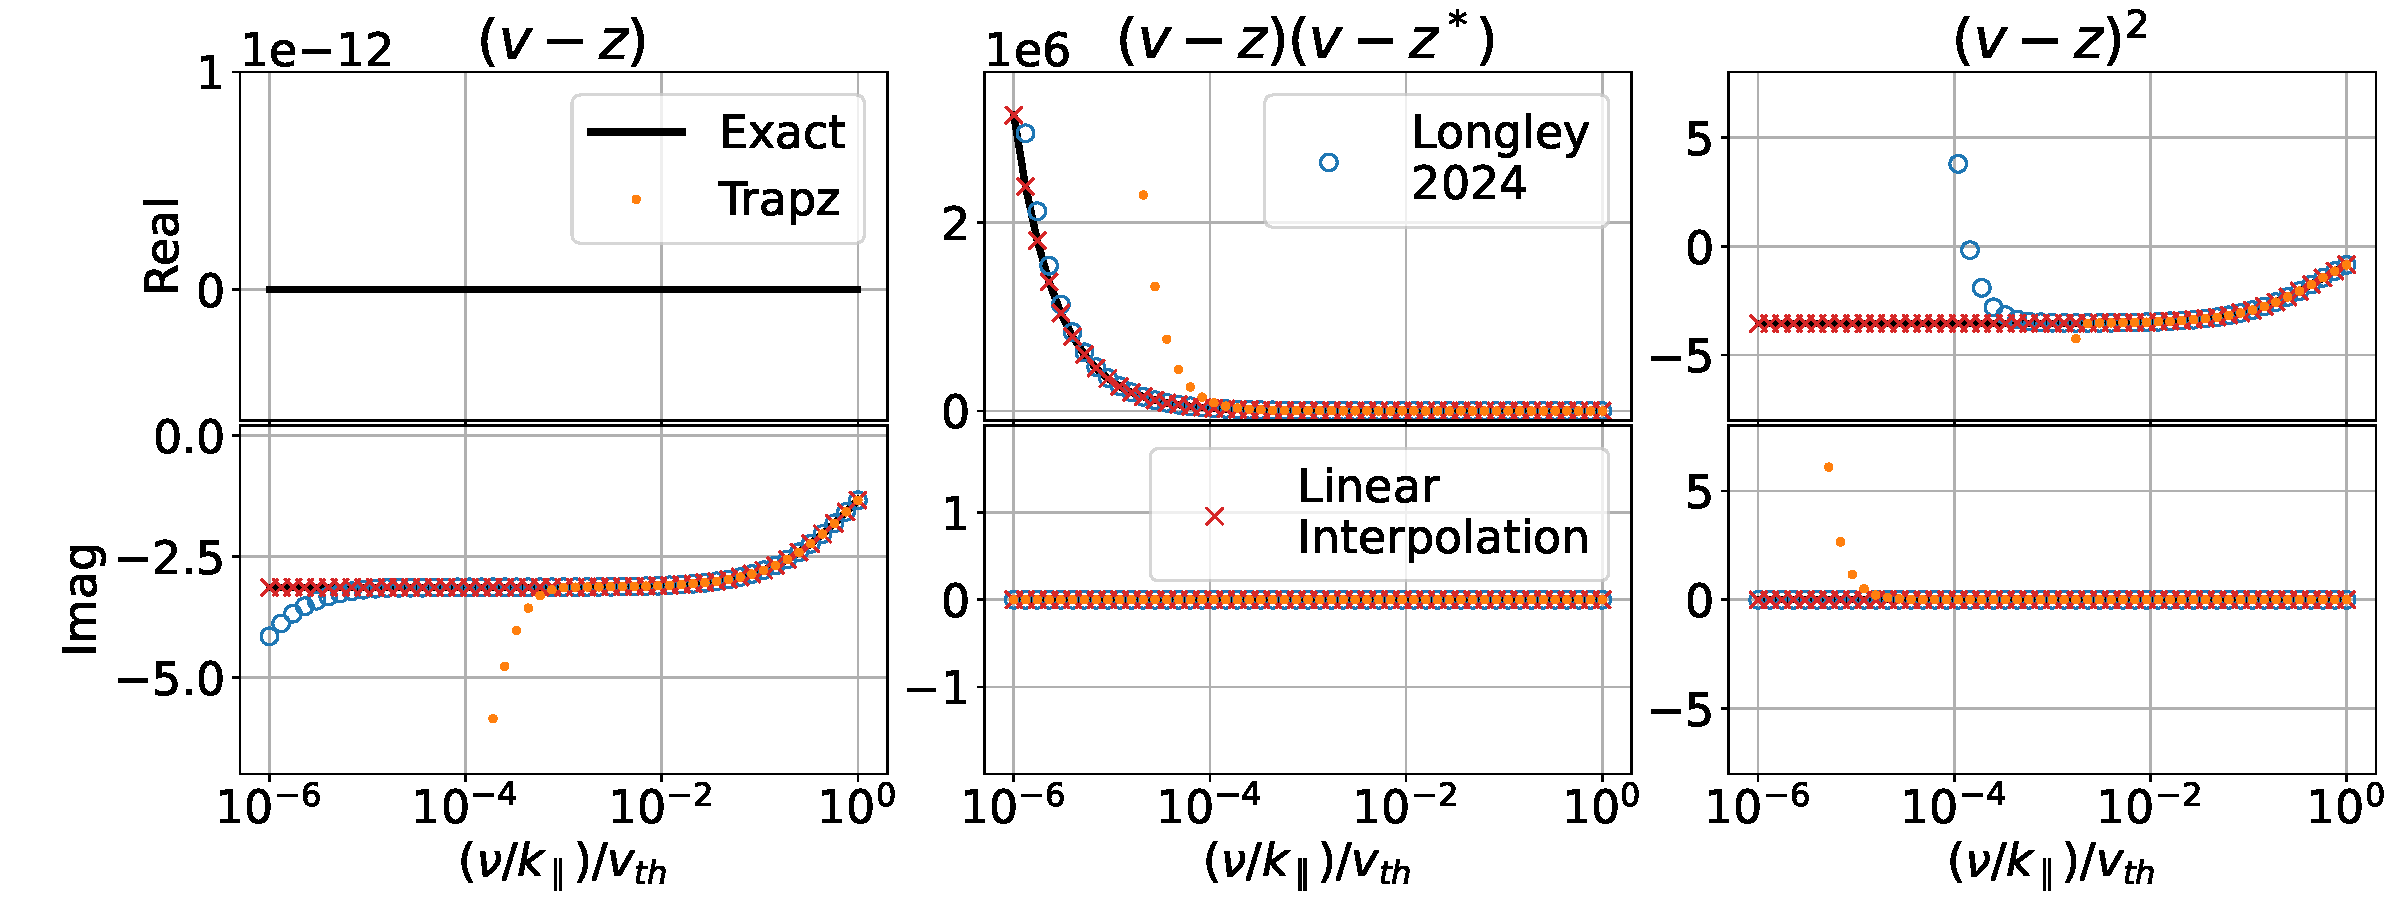
\includegraphics[width=\linewidth]{poleIntegrate_error_pole0_-3.pdf}
	\caption{Same as Fig.~\ref{f:poleIntegrateError0_pole0} but with $\Delta v_\parallel/v_{th}=10^{-3}$.}
	\label{f:poleIntegrateError-3_pole0}
\end{figure}

\begin{figure}[!htb]
	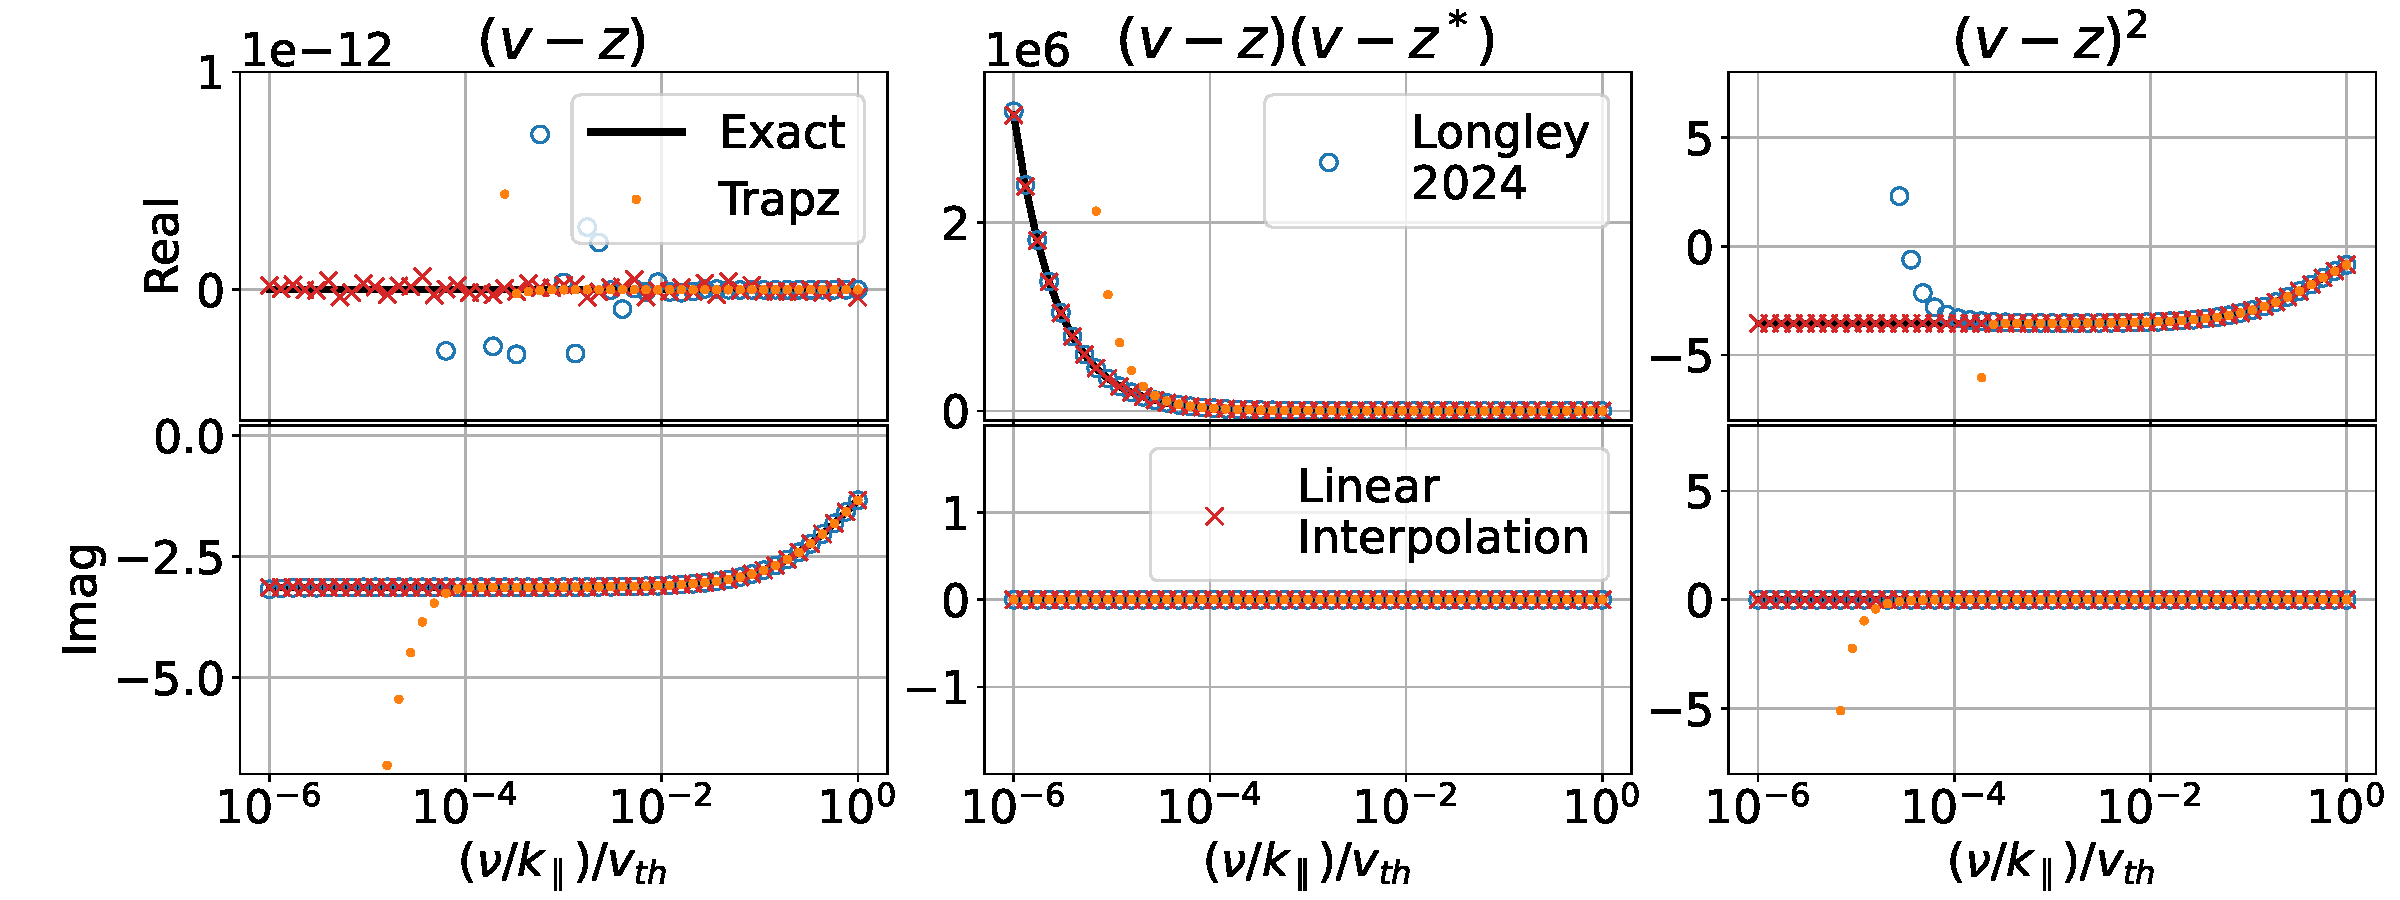
\includegraphics[width=\linewidth]{poleIntegrate_error_pole0_-4.pdf}
	\caption{Same as Fig.~\ref{f:poleIntegrateError0_pole0} but with $\Delta v_\parallel/v_{th}=10^{-4}$.}
	\label{f:poleIntegrateError-4_pole0}
\end{figure}

\begin{figure}[!htb]
	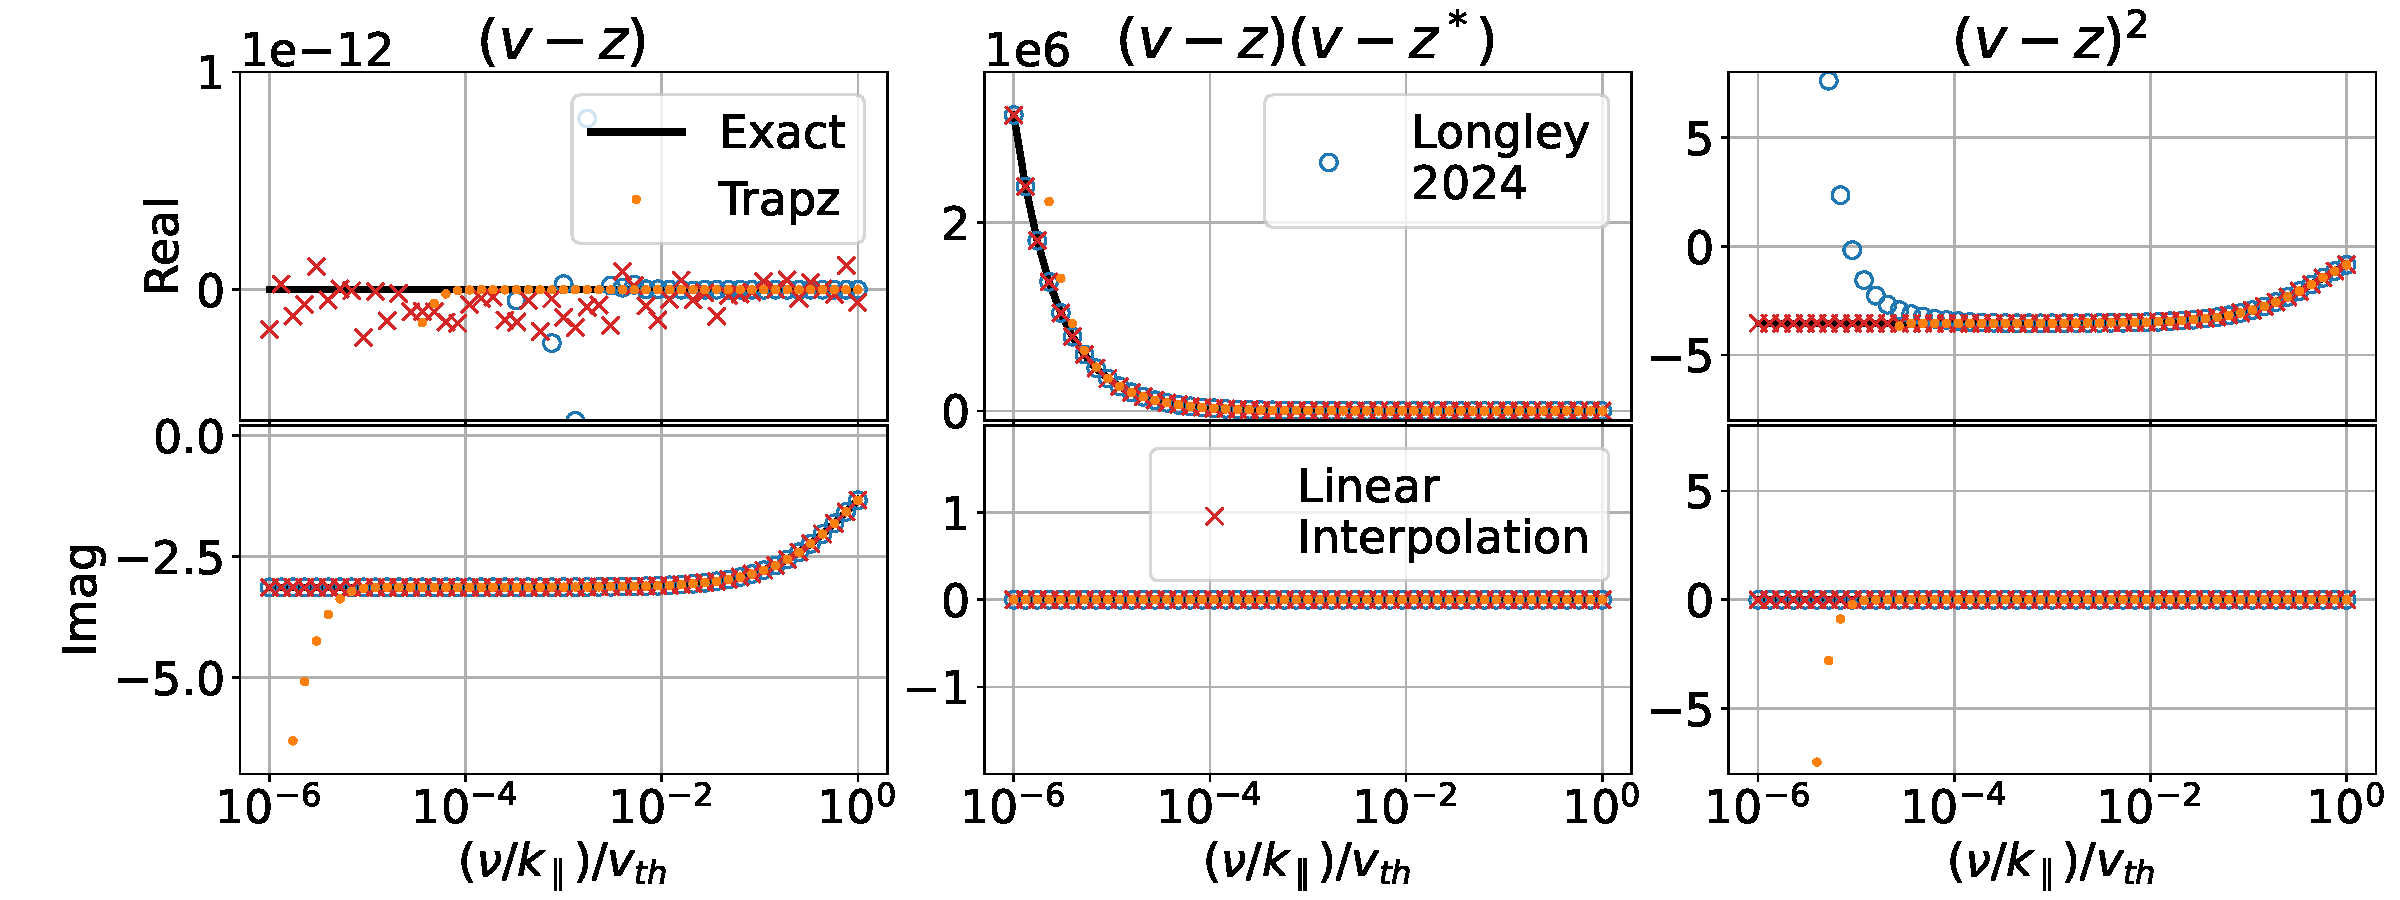
\includegraphics[width=\linewidth]{poleIntegrate_error_pole0_-5.pdf}
	\caption{Same as Fig.~\ref{f:poleIntegrateError0} but with $\Delta v_\parallel/v_{th}=10^{-5}$.}
	\label{f:poleIntegrateError-5_pole0}
\end{figure}


% Should we have a discussion somewhere about the merits of this method vs a quadrature approach? 
% I think one of the main pros to our method is that we don't need to worry beforehand about quadrature points and can have any arbitrary non-uniform mesh
% Further, to use quadrature, one needs to rewrite everything as Legendre polynomials yeah?
% If you are already doing it as a polynomial, then you can already use our method since it works for any arbitrary order polynomial. 
% I will show that somewhere too. The answer to these poles using the hypergeometric series solution from Mathematica. I first need to learn mroe and understand it though


\subsection{Extending to Arbitrary Polynomial Order}

Suppose instead of obtaining the distribution function as a discrete set of points (as one would in outputs of Monte Carlo, PIC, or finite discretization methodss), we have a solution with a polynomial representation (like those of spectral, Galerkin, and discontinuous Galerkin methods). 
For this work, we will only consider a discontinuous Galerkin approach, but the idea should is easily extended to global spectral represenations of the distribution function.
Consider a set of piecewise polynomial representations of the distribution as
\begin{equation}
	f_{0s,j}(v_\perp, v_\parallel) = c_0(v_\perp) + c_1(v_\perp) v_\parallel + c_2(v_\perp) v_\parallel^2 + \cdots + c_n(v_\perp) v_\parallel^n,
	= \sum_{m=0}^n c_m(v_\perp) v_\parallel^m
	\label{eq:arb_poly_dist} 
\end{equation}
where $c_j(v_\perp)$ are the polynomial coefficients for a polynomial of order $n$. 
Note that these coefficients are still functions of $v_\perp$ since we are only doing the pole integration in the parallel direction.
Thus, we can split the integral of the distribution function at some pole (we will use Eq.~\ref{eq:p1} as an example) into $n$ different integrals:
\begin{equation}
	\int \frac{f_{0s,j}(v_\perp, v_\parallel)}{v_\parallel -z} dv_\parallel = 
	\sum_{m=0}^n c_m(v_\perp)\int \frac{v_\parallel^m}{v_\parallel -z} dv_\parallel.
\end{equation}
 
In a similar way to Eqs.~\ref{eq:p1j}-\ref{eq:p2j}, we can obtain the indefinite integrals for each of these poles using the representation of the distribution function in Eq.~\ref{eq:arb_poly_dist} as
\begin{equation}
	p_1^j(v_\perp,v_\parallel) = \int \frac{f_{0s,j}(v_\perp, v_\parallel)}{v_\parallel-z} dv_\parallel = 
	\sum_{m=0}^n c_m(v_\perp) \frac{v_\parallel^{m+1}}{(m+1)z} \ _2F_1\bigg(1, m+1; m+2; \frac{v_\parallel}{z}\bigg)
	\label{eq:p1j_arb_poly}
\end{equation}
\begin{multline}
	p_*^j(v_\perp,v_\parallel) = \int \frac{f_{0s,j}(v_\perp, v_\parallel)}{(v_\parallel-z)(v_\parallel-z^*)} dv_\parallel \\
	= \sum_{m=0}^n c_m(v_\perp)
	\frac{v_\parallel^{m+1}}{2 i (m+1) |z|^2 \im(z)} 
	\Bigg[z \ _2F_1\bigg(1, m+1; m+2; \frac{v_\parallel}{z^*}  \bigg)  - z^* \ _2F_1\bigg(1, m+1; m+2; \frac{v_\parallel}{z}  \bigg)\Bigg]
	\label{eq:pstarj_arb_poly}
\end{multline}
\begin{equation}
	p_2^j(v_\perp,v_\parallel) = \int \frac{f_{0s,j}(v_\perp, v_\parallel)}{(v_\parallel-z)^2} dv_\parallel = 
	\sum_{m=0}^n c_m(v_\perp) \frac{v_\parallel^{m+1}}{(m+1)z^2} \ _2F_1\bigg(2, m+1; m+2; \frac{v_\parallel}{z}\bigg),
	\label{eq:p2j_arb_poly}
\end{equation}
where $_2F_1(a, b; c; z)$ is the hypergeometric function. % rethink how I want to say this.
% Add how to do this in python briefly

Track down how other people have done the plasma dispersion relation calculation and see what their applications have been for.



\subsection{Calculating temperature in arbitrary direction}
\label{s:equiv-temp-known}

This section discusses numerical methods used to calculate the temperature in an arbitrary direction.
From a practical perspective, we can use this to get the line of sight temperature, which is what a radar will see.
For an arbitrary distribution function, we can back out the temperature from its zeroth, first, and second moments in the line of sight velocity direction, $k$:
\begin{align}
	M_0 &= \int f d\mathbf{v} \label{eq:M0}\\
	M_{1_k} &= \int v_k f d\mathbf{v} \label{eq:M1} \\
	M_{2_{kk}} &= \int v_k^2 f d\mathbf{v}. \label{eq:M2}
\end{align}
From Eq.~\ref{eq:M0}-\ref{eq:M2}, we can calculate the temperature (assuming $v_{th}=\sqrt{2k_BT_k/m}$) in the line of sight direction as
\begin{equation}
	T_k = \frac{m}{k_B} \Bigg[ \frac{M_{2_{kk}}}{M_0}  - \bigg( \frac{M_{1_k}}{M_0} \bigg)^2\Bigg].
	\label{eq:Tk_full}
\end{equation}
For a Maxwellian distribution, you will find that this exactly backs out the temperature.
For a non-Maxwellian distribution, this will find the line of sight temperature equivalent (temperature can become ill defined for non-Maxwellian distributions).
In our case, we are using normalized distribution functions such that their zeroth moment (Eq.~\ref{eq:M0}) is 1 yielding
\begin{equation}
	T_k = \frac{m}{k_B} (M_{2_{kk}} - M_{1_k}^2).
	\label{eq:Tk_simp}
\end{equation}
All of our distributions we will be looking at are azimuthally symmetric. 
Furthermore, most (if not all) of the distributions we will consider are symmetric about the perpendicular plane where $v_\parallel=0$.
In this case, the first moment (Eq.~\ref{eq:M1}) is 0 giving an even further simplified 
\begin{equation}
	T_k = \frac{m M_{2_{kk}}}{k_B}.
	\label{eq:Tk_full_simp}
\end{equation}
Thus, all we need to do is figure out how to calculate the second moment in the line of sight direction.

\subsubsection{Known Distribution Function}
If we already know the functional form of the distribution function, then we can do some coordinate transformations to properly calculate Eq.~\ref{eq:Tk_full_simp}. 
Assume we have a Cartesian grid with coordinates $v_x$, $v_y$, and $v_z$.  % Have a pic of this in here eventually
Since we are only looking at azimuthally symmetric distribution function, it is convenient to use cylindrical coordinates in the form of $v_\parallel$ and $v_\perp$ with the directions being respective to the magnetic field.
For simplicity, let us assume that the parallel direction is in the direction of $v_z$.
Let us now consider a different coordinate system we call $v_x'$, $v_y'$, and $v_z'$ with $v_z'$ being in the line of sight direction.


Our goal is to write the orignal $v_{x,y,z}$ system in terms of the $v_{x,y,z}'$ system. 
By azimuthal symmetry and since we only care about how the temperature varies with angle respective to the magnetic field, the prime coordinate system, $v_{x,y,z}'$, is just a rotation of the original coordinate system, $v_{x,y,z}$, by $-\theta$ about the $v_x$ axis. 
Thus, to go the other way, the original coordinate system, $v_{x,y,z}$ can be found by rotating the prime coordinate system, $v_{x,y,z}'$, by $\theta$ about the $v_x'$ axis.
The standard rotation matrix for such a transformation is
\begin{equation}
	\mathbf{R}_{v_x}(\theta) = \begin{bmatrix}
		1 & 0 & 0 \\
		0 & \cos\theta & -\sin\theta \\
		0 & \sin\theta & \cos\theta
	\end{bmatrix}.
	\label{eq:rot_mat}
\end{equation}
Therefore, we can write the original coordinate system, $v_{x,y,z}$ in terms of the prime system, $v_{x,y,z}'$ as
\begin{equation}
	\begin{bmatrix}
		v_x \\ v_y \\ v_z
	\end{bmatrix} = 
	\mathbf{R}_{v_x} \begin{bmatrix}
		v_x' \\ v_y' \\ v_z'
	\end{bmatrix} = 
	\begin{bmatrix}
		v_x' \\
		v_y'\cos\theta - v_z'\sin\theta \\
		v_y'\sin\theta + v_z'\cos\theta
	\end{bmatrix}.
\end{equation}
Now, we must convert to cylindrical coordinates. 
We set $v_z$ to be in the parallel direction; therefore,
\begin{equation}
	v_\parallel = v_z = v_y'\sin\theta + v_z'\cos\theta.
\end{equation}
The perpendicular direction is just the radius giving
\begin{equation}
	v_\perp = \sqrt{v_x^2+v_y^2}
	= \sqrt{v_x'^2 + (v_y'\cos\theta - v_z'\sin\theta)^2 }.
\end{equation}
Based on these, we can effectively write any function of $v_\perp$ and $v_\parallel$ in terms of $v_{x,y,z}'$.
Thus, the second moment in the line of sight direction ($v_z'$) becomes
\begin{equation}
	M_{2_{z'z'}} = \int v_z'^2 f d\mathbf{v}'.
\end{equation}


\subsubsection{Unknown Distribution Function}

